%----------------------------------------------------------------------------------------
%----------------------------------------------------------------------------------------
%----------------------------------------------------------------------------------------
%Results
%----------------------------------------------------------------------------------------
%----------------------------------------------------------------------------------------
%----------------------------------------------------------------------------------------
\section{RESULTS and DISCUSSION}
\label{sec: result}

    In this section we show the results of the neural networks trained using the 12 \citetalias{Kinney96} template spectra.
    Training with \citetalias{Kinney96} templates results in networks that have regions corresponding to galaxies of known morphological type. 
    The trained networks can then be used to categorize other galaxies.
   
    In order to find a sufficient size for the trained networks, we created maps with sizes ranging from $1\times2$ to $50\times50$.
    Varying the grid size of the maps helped us to monitor whether tighter grouping of galaxies happens due to their similar properties or a lack of map space to separate them.
    Based on the size of the data and SOM results, we found the optimum grid size to be $1\times22$ and $12\times12$ in 1D and 2D maps, respectively. 
    For each grid we created different SOMs with different learning factors, neighbourhood distances, and number of iterations to find the most suitable values for our dataset, which are listed in Section~\ref{sec: create_som}. 
    
    We started our analysis by creating 1D SOMs. 
    First, we created SOMs with only two neurons ($1\times2$ map), and then increased the number of neurons one at a time in the 1D case (Sec.~\ref{sec: 1D}).
    We generate 2D networks (Sec.~\ref{sec: 2D}),  again starting with the smallest possible number of neurons (4 neurons in a $2\times2$ map), increasing to 144 in a $12\times12$ map.    
    For each generated network, we compare the results with the \citetalias{Kinney96} categorization.
    We also use these networks to classify the \citetalias{Hossein12} galaxy sample, and compare this classification with that from the supervised networks in \citetalias{Hossein12}.

    \subsection{One-dimensional self-organizing maps}
    \label{sec: 1D}
        \subsubsection{TRAINING THE NETWORKS}
        \label{sec: 1Dt}
            To start our clustering, we assumed that galaxies can be divided into only two general types: quiescent and starburst.
            This corresponds to a network with only two neurons.
            We increased the size of the map gradually until the 12 input samples divide into the 12 neurons. 
        
            Figs.~\ref{fig: 1by2T} --\ref{fig: 1by22T}~show the results of the training $1\times2$, $1\times3$, and $1\times22$ networks, respectively (the remaining networks are shown in Appendix~\ref{app: high_Z_1d_soms}).
            As in Fig.~\ref{fig: sample}, the upper part of the figures shows the neurons and their relative distances, $D_j$.
            As mentioned in Sec.~\ref{sec: method}, an increase in the darkness of colours between neurons represents an increase in relative distance between the neurons.
            The lower panels of the figures show the number of \citetalias{Kinney96} templates that are placed in each neuron. 
            \begin{figure}
                \begin{subfigure}[b]{0.5\textwidth}
                    \centering
                    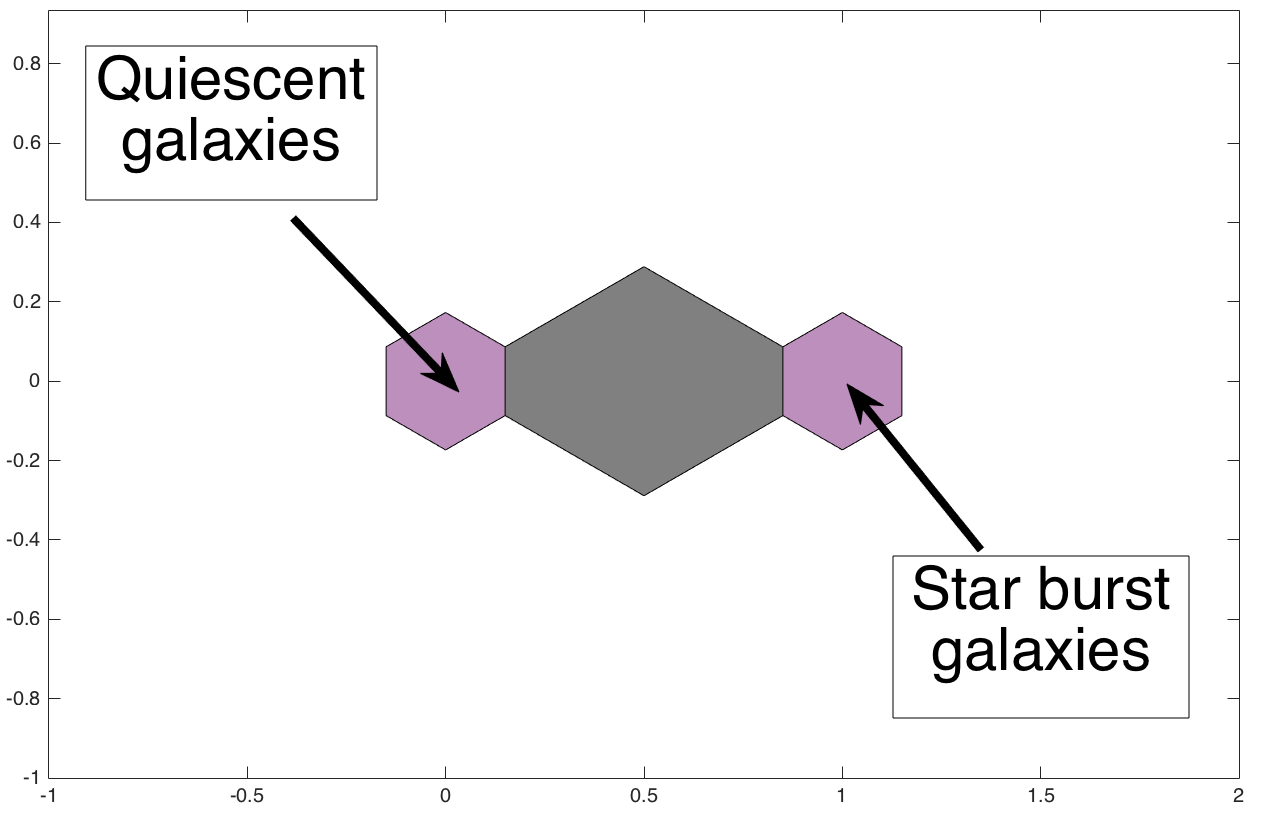
\includegraphics[width=\textwidth]{images0.01/1d/dist_1_by_2.png}
                \end{subfigure}
                \hfill
                \begin{subfigure}[b]{0.5\textwidth}
                     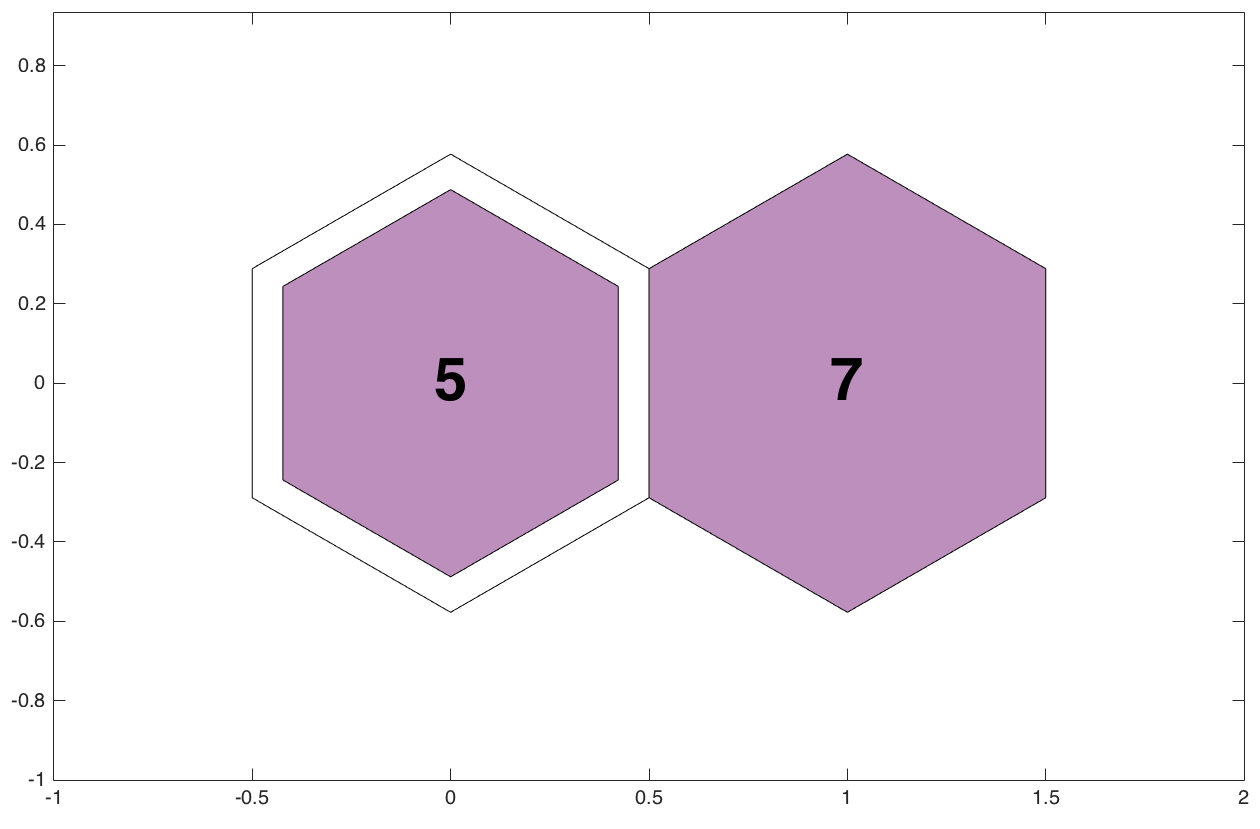
\includegraphics[width=\textwidth]{images0.01/1d/hit_t_1_by_2.png}
                \end{subfigure}
                \caption{Results of training network in $1\times2$~grid. As in Fig.~\ref{fig: sample}, the upper panel is a distance map and the lower panel is a hit map. In this network, 5 of the templates from \citetalias{Kinney96} are categorized as quiescent galaxies and the rest are starbursts. Because of their strong emission lines, Sc galaxies are moved towards the starburst ones.}
                 \label{fig: 1by2T}
            \end{figure}
        
        
            In the upper map in Fig.~\ref{fig: 1by2T}, the dark colour between two neurons indicates that the relative distance between these two groups are relatively high, and these two groups are distinguishable groups.
            In the lower part of Fig.~\ref{fig: 1by2T}, we see that the templates are divided into two groups of 5 and 7.
            Although we know from \citetalias{Kinney96} and \citetalias{Hossein12} that 6 of the templates are quiescent and the other 6 are starbursts, the SOM results show 5 of the galaxies in one group and the other 7 in the second group.
            In this method, the Sc template has been categorized as starburst due to the relatively higher disk stellar population compared to that of the bulge. 
            According to \citetalias{Kinney96}, Sc galaxies are considered to be late Hubble type galaxies which have a flatter SED compare to other quiescent galaxies. 
            

            Fig.~\ref{fig: 1by3T} shows the results of the training in a 1$\times$3 network.
            In these plots we force the galaxies to be categorized in a maximum of 3 groups. 
            If the templates in Fig.~\ref{fig: 1by2T} truly belonged in two groups, they would be grouped into two groups in this network, even when we try to cluster them into three. 
            However, in the lower panel of Fig.~\ref{fig: 1by3T}, we can see that the middle node contains two templates.
            These two templates, which are separated from the group of starburst templates in the lower part of Fig.~\ref{fig: 1by2T},  are the SB5 and SB6 types.
            In the upper plot of Fig.~\ref{fig: 1by3T}, the colour between two right neurons is black and the colour between two left neurons is white. 
            The black colour indicates that the left neuron is completely different from the other two groups,
            while the white colour shows that the two right neurons are very similar to one another. 
            
            Comparing Fig.~\ref{fig: 1by2T} to Fig.~\ref{fig: 1by3T} shows that the starburst templates are divided into two groups. 
            Based on the colours between these two groups, we conclude that they are very similar; both groups are starbursting and have strong emission lines.
            On the other hand, the SB5 and SB6 templates have the highest internal extinctions; this causes the SED to become flatter at shorter wavelengths. 
            The flatter UV SED makes these two templates more similar to quiescent galaxies than to other starbursts.
            Therefore, in the networks, SB5 and SB6 types are to be grouped close to the early type galaxy templates.
                
            \begin{figure}
                \begin{subfigure}[b]{0.5\textwidth}
                    \centering
                    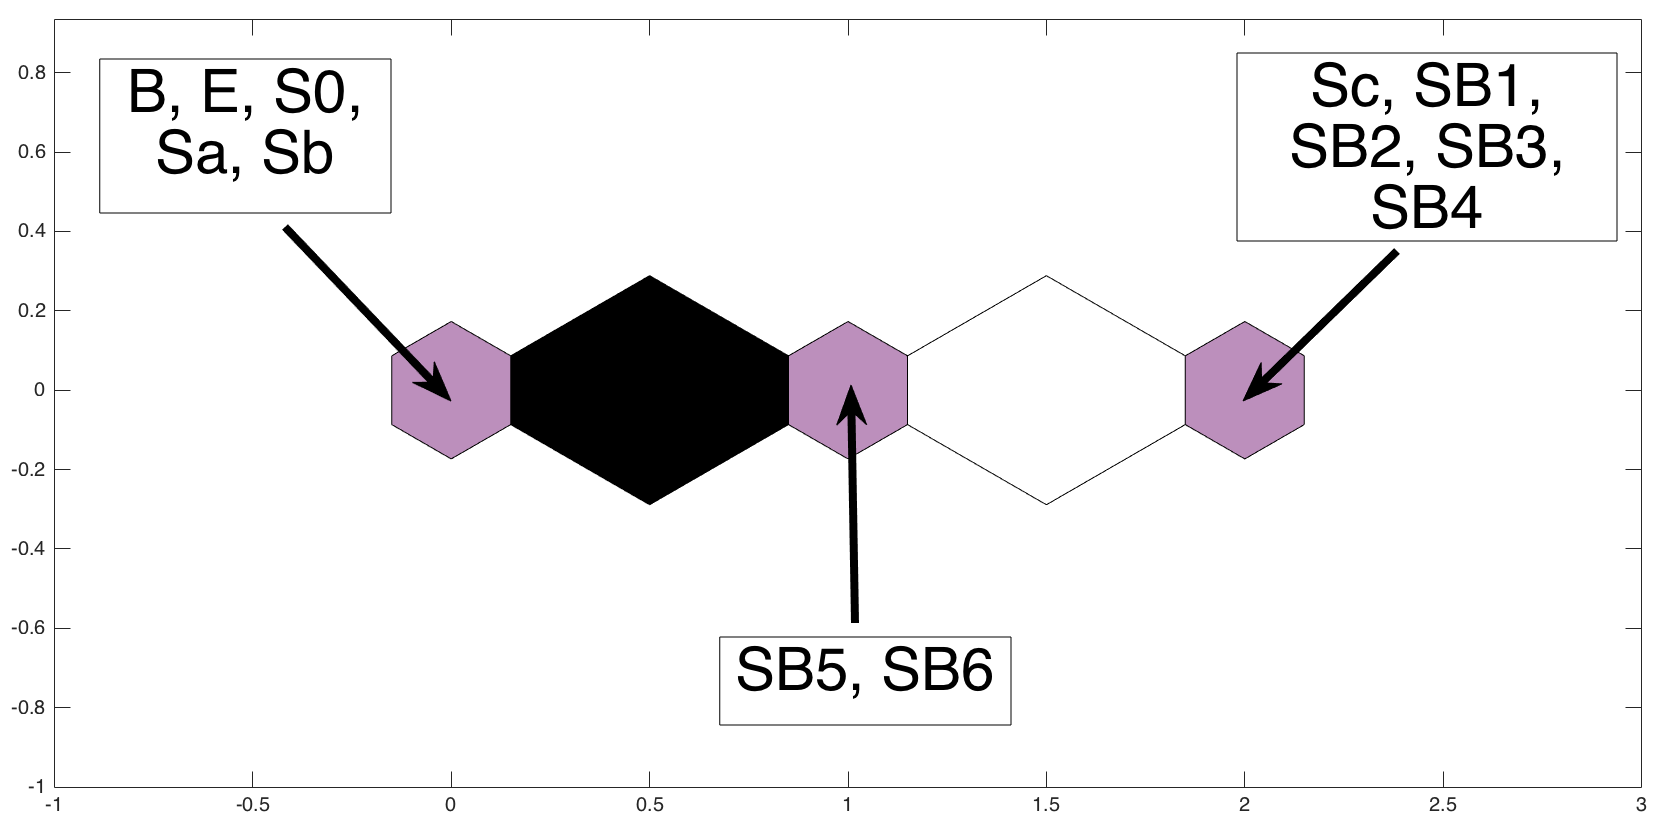
\includegraphics[width=\textwidth]{images0.01/1d/dist_1_by_3.png}
                \end{subfigure}
                \hfill
                \begin{subfigure}[b]{0.5\textwidth}
                     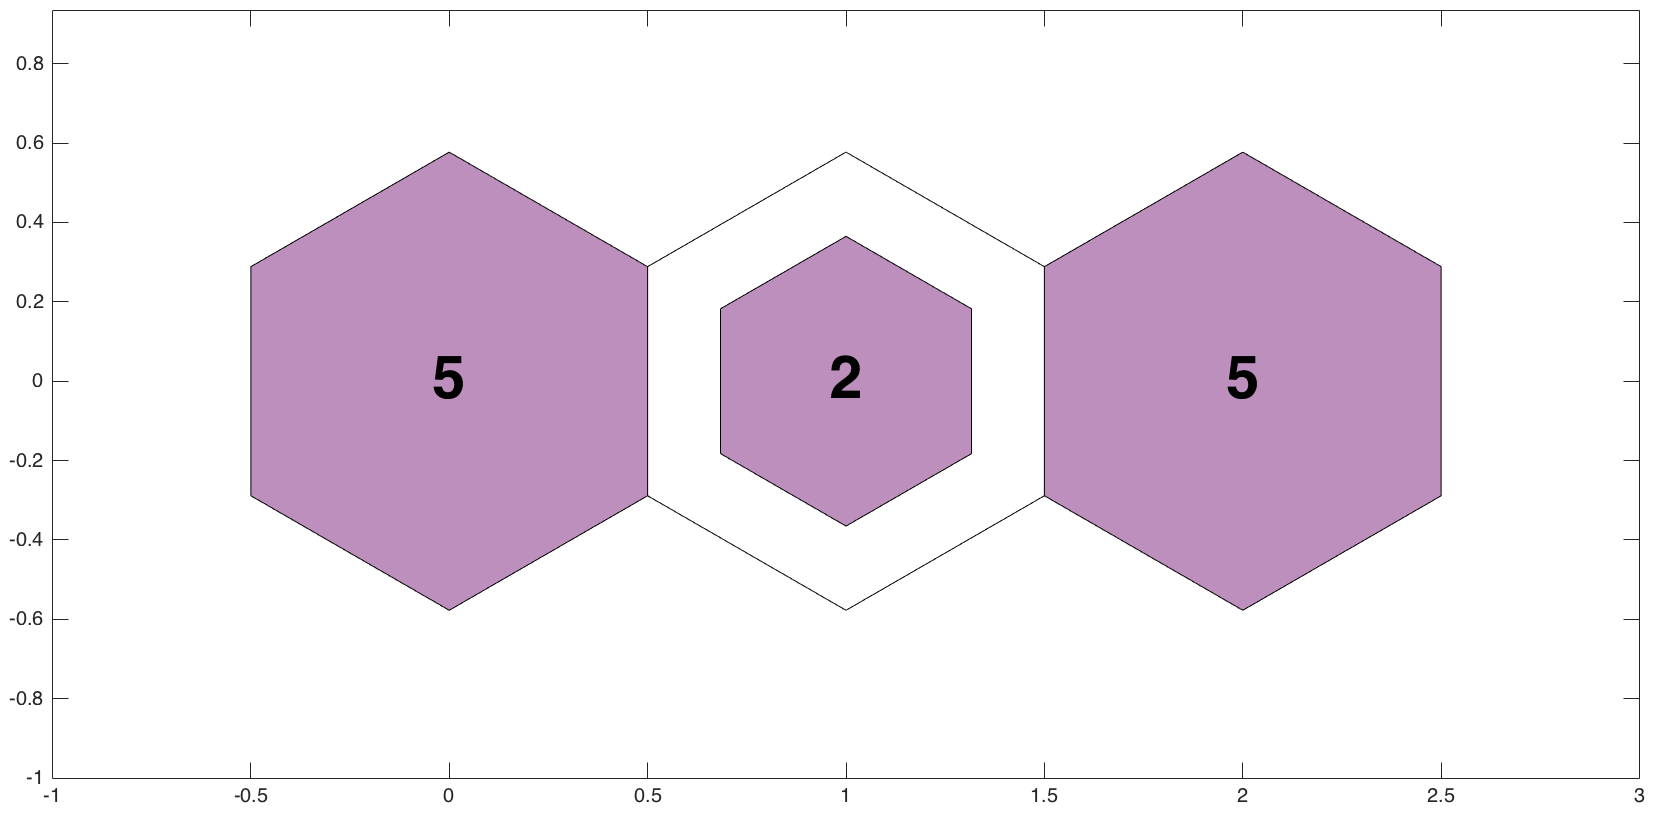
\includegraphics[width=\textwidth]{images0.01/1d/hit_t_1_by_3.png}
                \end{subfigure}
                \caption{The same as Fig.~\ref{fig: 1by2T} but showing the results of training network in $1\times3$~grid. In this network again, 5 of the \citetalias{Kinney96} templates are categorized as quiescent and 7 as starbursts. However, this time 2  templates (SB5 and SB6) are separated from the starburst groups.}
                 \label{fig: 1by3T}
            \end{figure}
           
            We increased the size of the maps gradually until the galaxies are divided into twelve groups (Figs.~\ref{fig: 1by4T} to ~\ref{fig: 1by20T} and ~\ref{fig: 1by22T}).
            Since there are more nodes in larger SOMs, the  algorithm 
            pays more attention to small differences between groups.
            If the templates from \citetalias{Kinney96} had completely distinct SEDs, then a $1\times12$-sized SOM would be expected to show 12 different groups each containing a single template.
            However, in Fig.~\ref{fig: 1by12T}, we see that three of the neurons contain two templates and three of them are empty.
            It is evident that there was no template in the \citetalias{Kinney96} sample that can fill those empty neurons.
            In Fig.~\ref{fig: 1by12T}, from left to right, templates with types B and E, SB3 and SB4, and SB1 and SB2 are the ones grouped together. 
            The SB3 and SB4 grouping breaks when we increase the size of the network to $1\times15$~(Fig.~\ref{fig: 1by15T}).
            The SB1 and SB2 templates, however, remain in the same neuron until the size of the map is increased to $1\times20$~(Fig.~\ref{fig: 1by20T}).
            The separation between templates B and E only happens when the size of the SOM exceeds $1\times22$~(Fig.~\ref{fig: 1by22T}).
        \begin{figure*}
            \begin{subfigure}[b]{\textwidth}
                \centering
                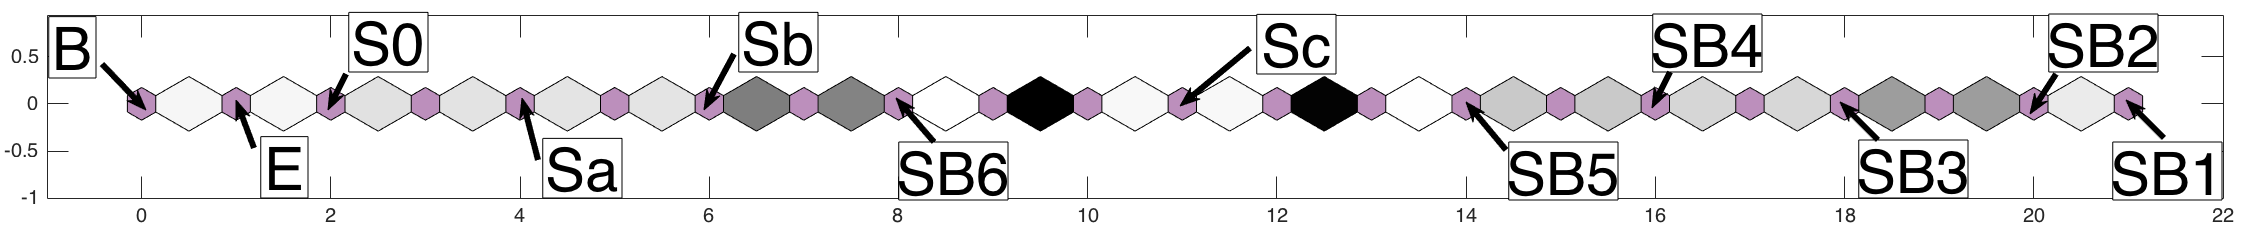
\includegraphics[width=\textwidth]{images0.01/1d/dist_1_by_22.png}
            %\caption{$1\times22$ weight map}
             %\label{fig: 1by22T}
            \end{subfigure}
            \hfill
            \begin{subfigure}[b]{\textwidth}
                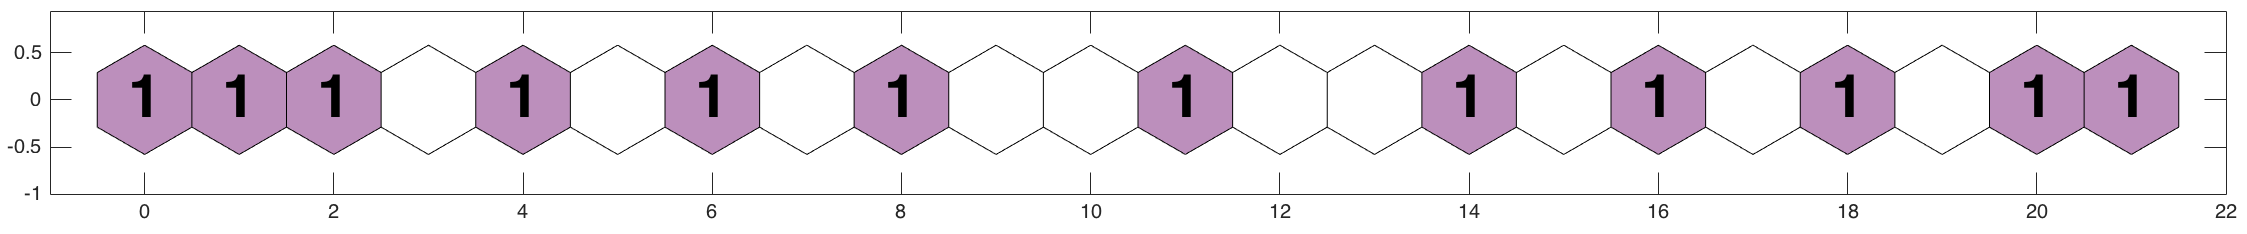
\includegraphics[width=\textwidth]{images0.01/1d/hit_t_1_by_22.png}
             %\caption{$1\times22$ hits map}
             %\label{fig: 1by22Thits}
            \end{subfigure}
            \caption{The same as Fig.~\ref{fig: 1by2T} but this time the figure shows results of training network in $1\times22$~grid.}
            \label{fig: 1by22T}
        \end{figure*} %PB160427: this figure looks really great! Very easy to understand.
    
            In Fig.~\ref{fig: 1by22T}, we can see twelve different groups:
            5 groups in the left-side neurons are separated from 7 groups on the right side of the map with two dark-grey colours between them.
            This shows that even though the galaxies are clustered in twelve groups, there still remain only two main distinct groups.
            The closest occupied neuron in the starburst side of the SOM, belongs to the SB6 type. 
            This template has the most extinction and its SED has more similarity to early type galaxies than other starburst types. 
            
            The fact that the templates need to have at least 22 different neurons to be divided into 12 groups shows that the differences between SB1 and SB2, and B and E, templates are very small.
            Because of their similarities, they tend to stay in the same group until the network becomes big enough to make use of the smallest particularity.
           
        \subsubsection{Classifying the galaxy sample}
         \label{sec: 1Dv}
            After training the networks as discussed in Sec.~\ref{sec: 1Dt}, we used them to classify the fitted SEDs of the sample of 142 galaxies from \citetalias{Hossein12}.
            The upper panel in Fig.~\ref{fig: 1by2V} shows the result of this classification using the $1\times2$~network from Fig.~\ref{fig: 1by2T}.
            Eighty of the galaxies have SEDs similar to those of the early type galaxies and the SEDs of the rest are similar to the starburst galaxies.
            The lower left panel shows the average SED of the 80 galaxies that were classified as quiescent. 
            These galaxies are similar to the ones in the left node in the upper panel of Fig.~\ref{fig: 1by2T}:
            the SEDs clearly show the 4000\AA~break, one of the signatures of quiescent galaxies.
            The H$\alpha$ emission in the spectrum could be from galaxies with similar SEDs to Sa galaxies, but with stronger emission lines.
            The average SED in the lower right panel of Fig.~\ref{fig: 1by2V} shows strong emission lines and bright ultraviolet continuum, indications of a high star formation rate.
            \begin{figure}
                \begin{subfigure}[b]{0.5\textwidth}
                    \centering
                    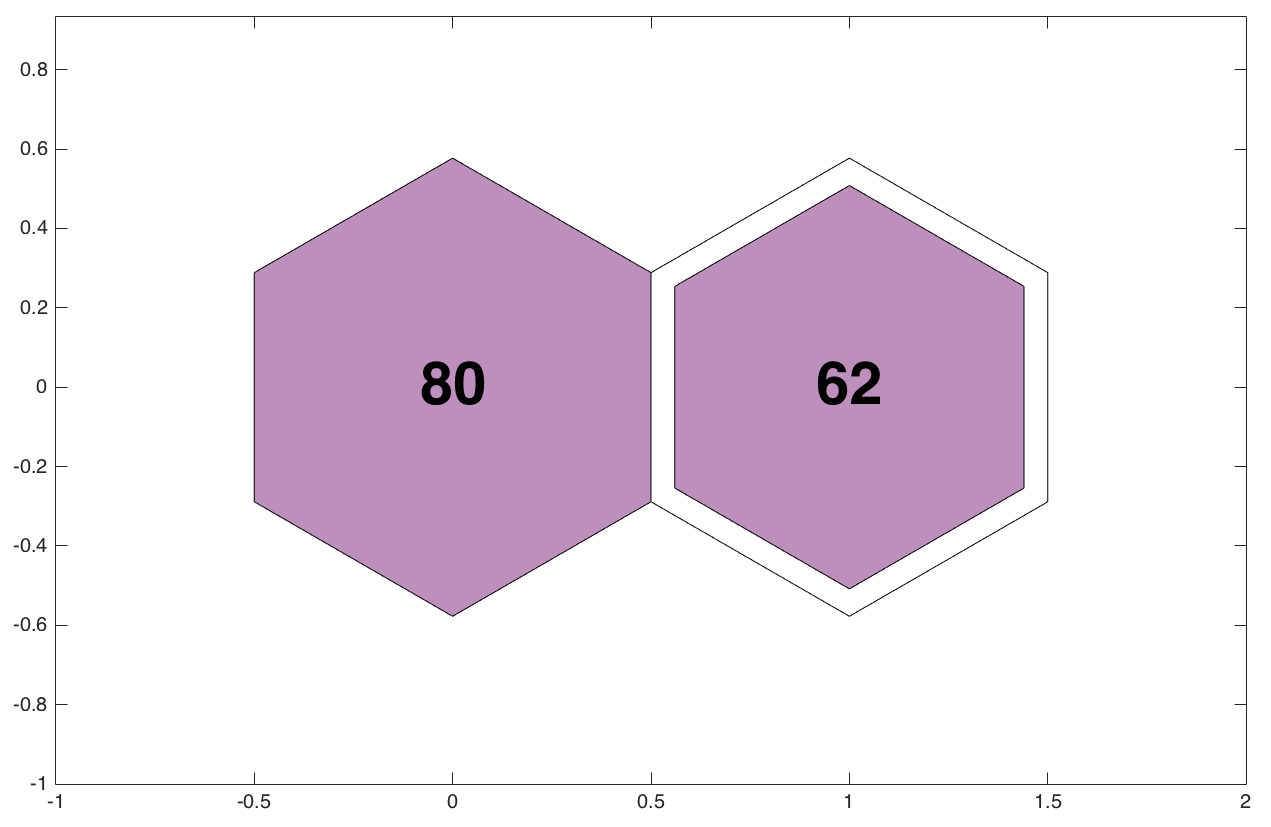
\includegraphics[width=\textwidth]{images0.01/1d/hit_v_1_by_2.png}
                    %\caption{$1\times2$ weight map}
                     %\label{fig: 1by3T}
                \end{subfigure}
                \hfill
                \begin{subfigure}[b]{0.5\textwidth}
                     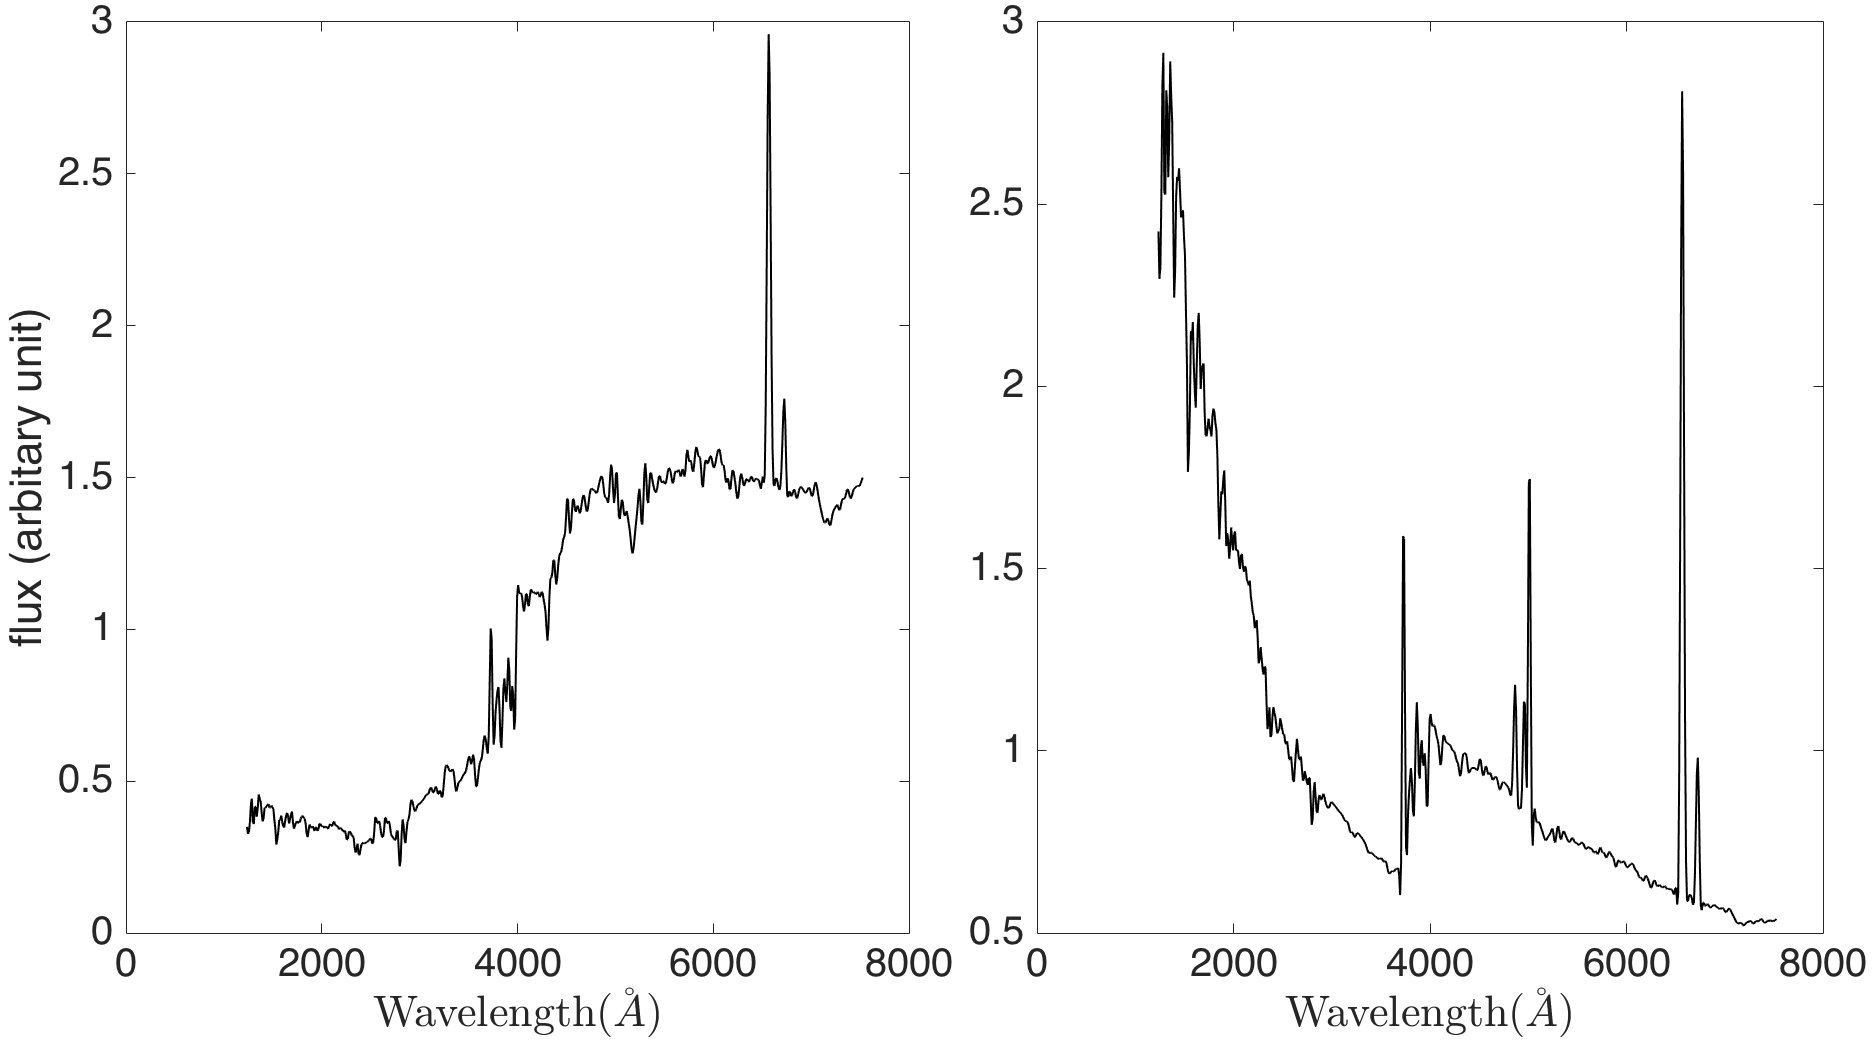
\includegraphics[width=\textwidth]{images0.01/1d/SED_total1by2.png}
                     %\caption{$1\times2$ hits map}
                     %\label{fig: 1by3Thits}
                \end{subfigure}
                \caption{Classification of fitted galaxy SEDs from \citetalias{Hossein12} using the $1\times2$~network trained from the \citetalias{Kinney96} templates (Fig.~\ref{fig: 1by2T}). Upper panel: a hit map with the number in each node representing the number of galaxies belonging to that group. In this case 80 means that 80 of the 142 SEDs are classified into the early type group while the 62 of the 142 SEDs are categorized as starburst galaxies. Lower panel: Average SED of the galaxies in each group, quiescent on the left and starburst on the right.}
                \label{fig: 1by2V}
            \end{figure}          
            
            Since in this network galaxies were forced to divide into a maximum of two groups, the strongest feature in a galaxy's SED predominantly decides which group the galaxy belongs to.
            Galaxies with a weak 4000\AA~break but strong emission lines and ultraviolet upturn are categorized as starbursts while galaxies with a strong 4000\AA~break are categorized as quiescent.
            Increasing the size of the SOM helps solve the problem of the galaxies which have features common to both groups.
            
            Fig.~\ref{fig: 1by3V} presents the result of classifying the SED of the galaxies using the $1\times3$~network (from Fig.~\ref{fig: 1by2T}): 66 of the galaxies belong to the early type group, and 47 belong to the starburst group. 
            However, 29 of the galaxies are similar to starbursts in some, but not all, of their features. 
            Galaxies in this group have strong emission lines and are ultraviolet-bright, but they also have a strong 4000\AA~break, which makes them cluster closer to the quiescent galaxies (middle panel in the lower part of Fig.~\ref{fig: 1by2V}).

            \begin{figure}
                \begin{subfigure}[b]{0.5\textwidth}
                    \centering
                    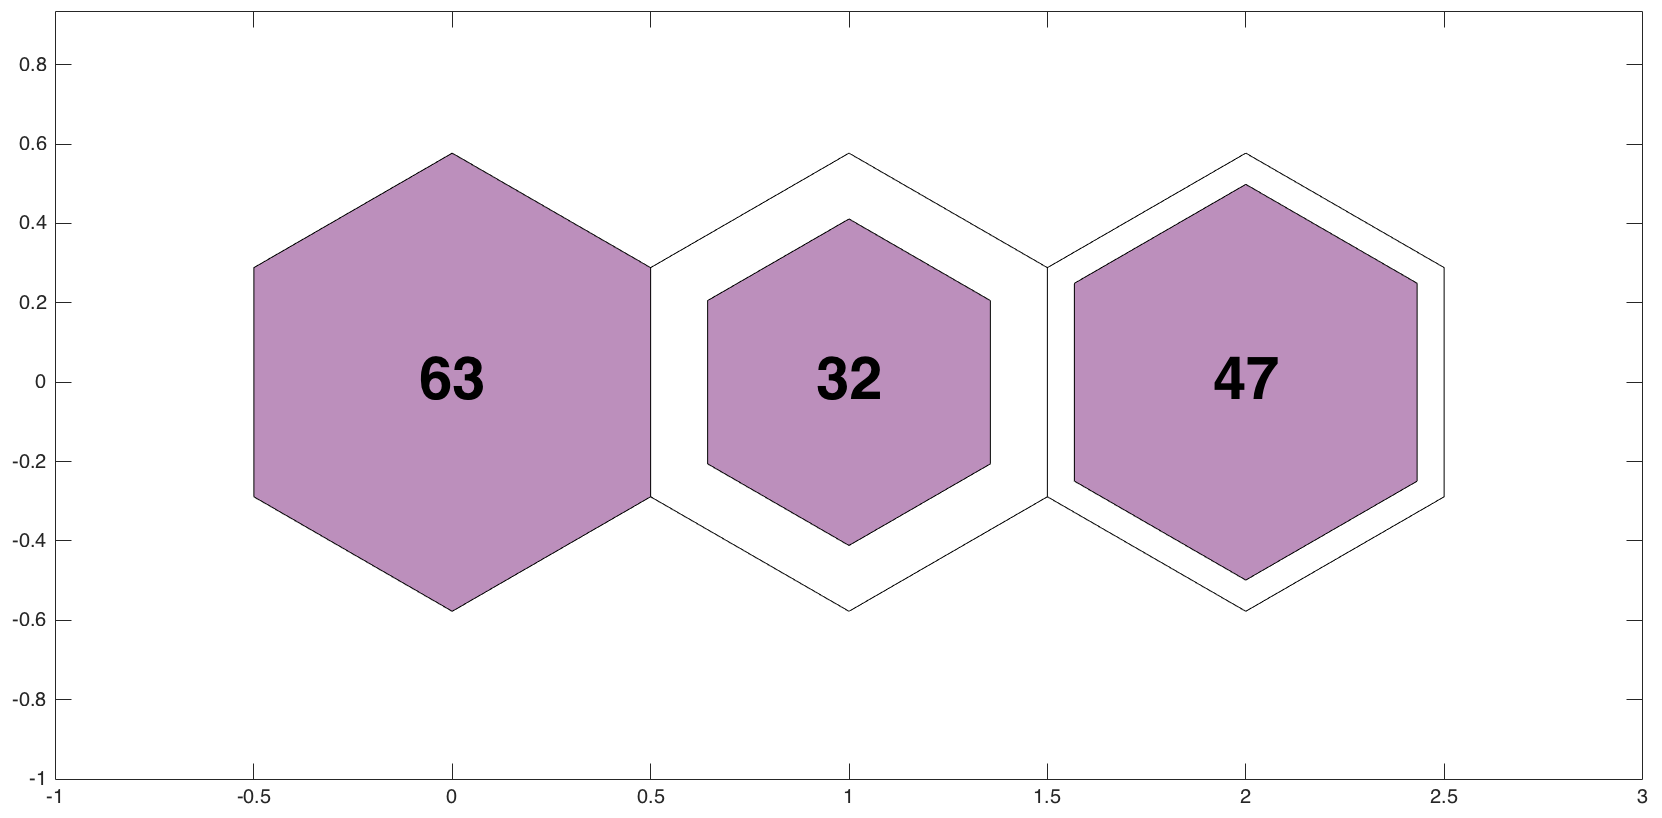
\includegraphics[width=\textwidth]{images0.01/1d/hit_v_1_by_3.png}
                    %\caption{$1\times2$ weight map}
                     %\label{fig: 1by3T}
                \end{subfigure}
                \hfill
                \begin{subfigure}[b]{0.5\textwidth}
                     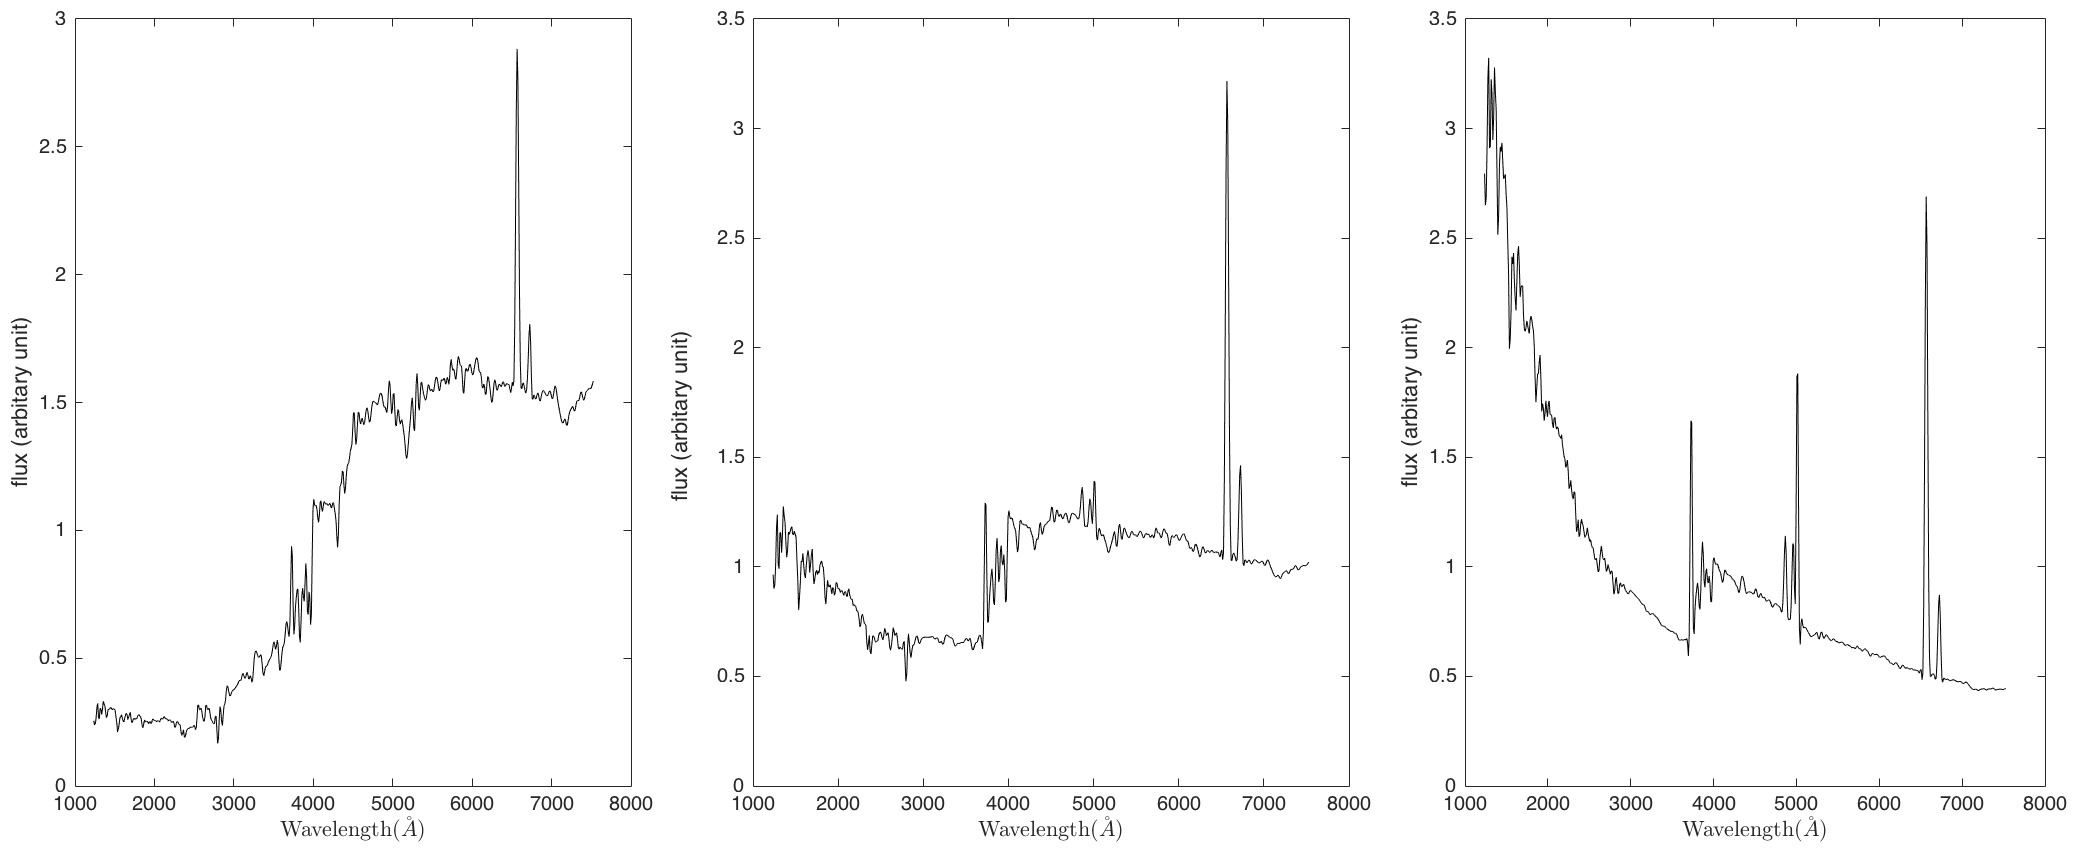
\includegraphics[width=\textwidth]{images0.01/1d/SED_total1by3.png}
                     %\caption{$1\times2$ hits map}
                     %\label{fig: 1by3Thits}
                \end{subfigure}
                \caption{Same as Fig.~\ref{fig: 1by2V}, but in this figure, we used a network with size of $1\times3$ (Fig.~\ref{fig: 1by3T}) to classify the sample galaxies.}
                \label{fig: 1by3V}
            \end{figure}       
            
            In Fig.~\ref{fig: 1by22V}, we use the $1\times22$~network to classify the sample galaxies.
            As mentioned in Sec.~\ref{sec: 1Dt}, in this network size we observed the first separation of the \citetalias{Kinney96} galaxies into 12 different neurons.
           As in Figs.~\ref{fig: 1by2V} and ~\ref{fig: 1by3V}, the upper panel of Fig.~\ref{fig: 1by22V} shows the number of galaxies (out of the 142) belonging to each neuron in the $1\times22$ SOM.
            \begin{figure*}
                \begin{subfigure}[b]{0.9\textwidth}
                    \centering
                    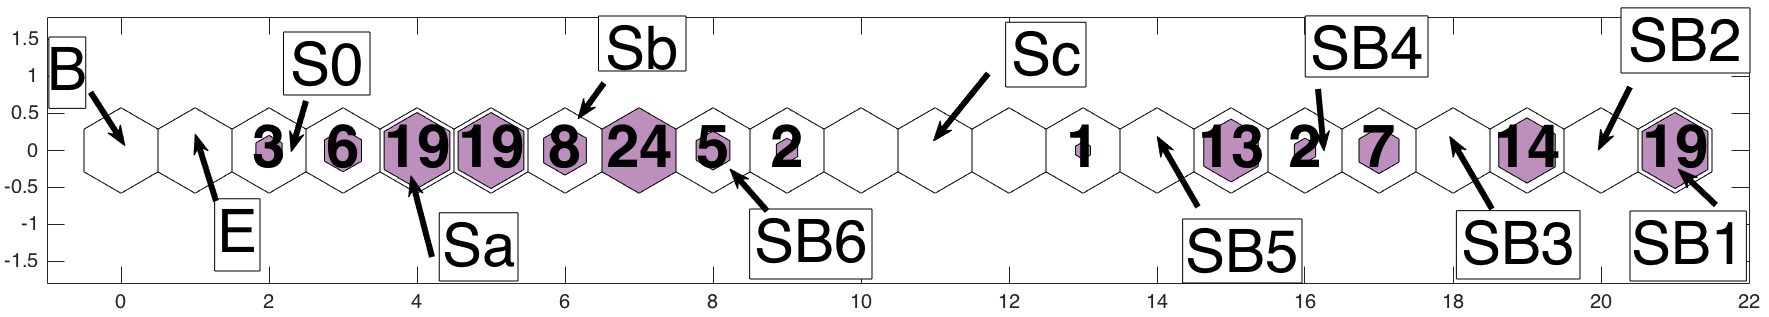
\includegraphics[width=\textwidth]{images0.01/1d/hit_v_1_by_22_n.png}
                    %\caption{$1\times2$ weight map}
                     %\label{fig: 1by3T}
                \end{subfigure}
                \hfill
                \begin{subfigure}[b]{0.9\textwidth}
                     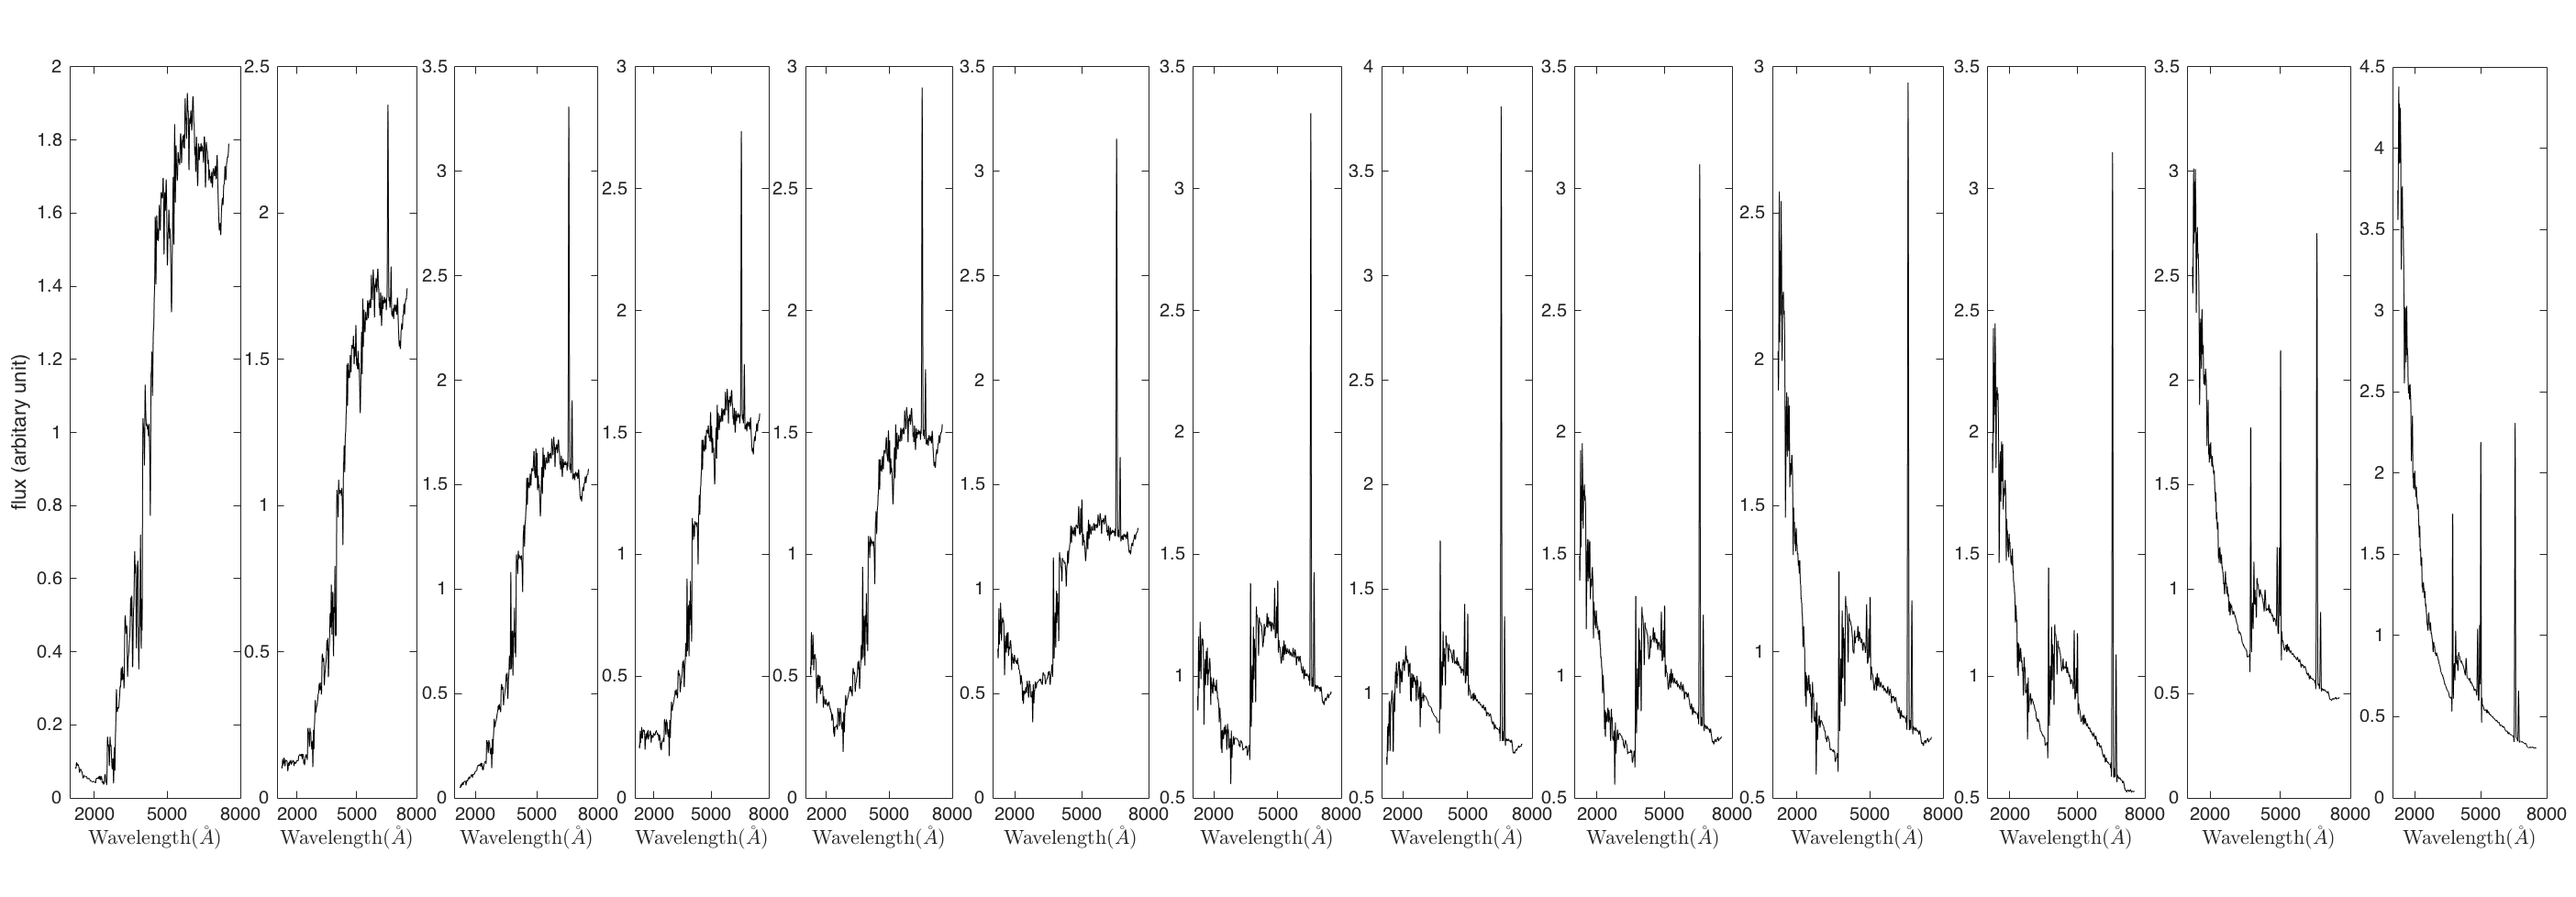
\includegraphics[width=\textwidth]{images0.01/1d/SED_total1by22.png}
                     %\caption{$1\times2$ hits map}
                     %\label{fig: 1by3Thits}
                \end{subfigure}
                \caption{Same as Fig.~\ref{fig: 1by2V}, but in this figure, we used a network with size of $1\times22$ (Fig.~\ref{fig: 1by22T}) to classify the sample galaxies. In the average SED of each neuron, we can clearly see the changes from early type galaxies to the starburst ones. The 4000\AA~ break weakens from left to right and the emission line strengths increase.}
                \label{fig: 1by22V}
            \end{figure*}
            The lower panels present the average SED of the galaxies in each neuron.
            Since galaxies had more space to separate, some of the neurons are left empty.
            Thus, instead of having 22 average SED plots in the lower part of Fig.~\ref{fig: 1by22V}, there are only 12.
            
            Comparing the upper panel of Fig.~\ref{fig: 1by22V} with the lower panel of Fig.~\ref{fig: 1by22T} shows that the occupied neurons are not necessarily the same.
            If a cluster from the \citetalias{Hossein12} sample fills the same neuron as a \citetalias{Kinney96} template, we can conclude that SEDs of galaxies in the cluster are very similar to those of the template.
            Otherwise, we can conclude that the SEDs of galaxies in the cluster are similar to two of the \citetalias{Kinney96} templates.
            For the latter case, the colours establish which template has greater similarity to the \citetalias{Hossein12} cluster.
            
            The first two neurons in the upper plot in Fig.~\ref{fig: 1by22V} are empty, while these neurons were occupied by galaxies B and E in the trained network.
            We therefore conclude that there are no galaxies in the \citetalias{Hossein12} sample with SEDs similar to that of type B or E.
            There are 3 galaxies in the third neuron, similar to the S0 type. 
            Eighteen of the galaxies are in the fifth neuron and similar to the Sa type, while the 7 galaxies in the fourth neuron have SEDs similar to both S0 and Sa galaxies.
            There is one Sb type galaxy and 15 galaxies with SEDs similar to both Sa and Sb type galaxies.
            The following two neurons (eighth and ninth neurons from the left) are on the edge of the early type and starburst galaxies.
            In the upper panel in Fig.~\ref{fig: 1by22T}, the colour between these two neurons is black, which shows that these two are very different.
            Therefore, 24 galaxies in the eighth neurons have similar SEDs to Sb type galaxies, and the SEDs of the 14 galaxies in the ninth neuron are similar to the SB6 galaxies.
            The far right neurons in the network belong to galaxies with SED comparable to types SB1 and SB2.
            
            In general, 56 galaxies correspond exactly to \citetalias{Kinney96} templates and the other 86 are placed between the initial 12 suggestions.
            As \citetalias{Hossein12} mentioned, part of the reason we could not classify all the galaxies using the \citetalias{Kinney96} model is that the model was constructed from co-adding spectra of 70 galaxies.
            In this small sample, it is quite possible that the best SEDs do not match any model perfectly and the original classifications have high uncertainties.
            
            Other methods for finding the type of galaxies (e.g. $\chi^2$ fitting and supervised neural network) are limited to templates: the outliers cannot be classified.
            However, using the SOM method we categorized galaxies based on their position on trained maps, which can have empty neurons.
            The empty neurons in a trained SOM show that there must be another type of template that is absent from the \citetalias{Kinney96} template spectra.
            Using the distance within the trained network is the best way to describe the properties of this absent template.
            Therefore, with SOM, we have the freedom to categorize galaxies in intermediate (new) templates.
       . 
        \subsubsection{PROPERTIES OF THE CLUSTERED GALAXIES}
        
        In order to check whether our clustering in Sec.~\ref{sec: 1Dv}~is correct, in this section we examine the relations between median properties of the galaxies in each neuron. 
        
        \begin{figure}
            \centering
            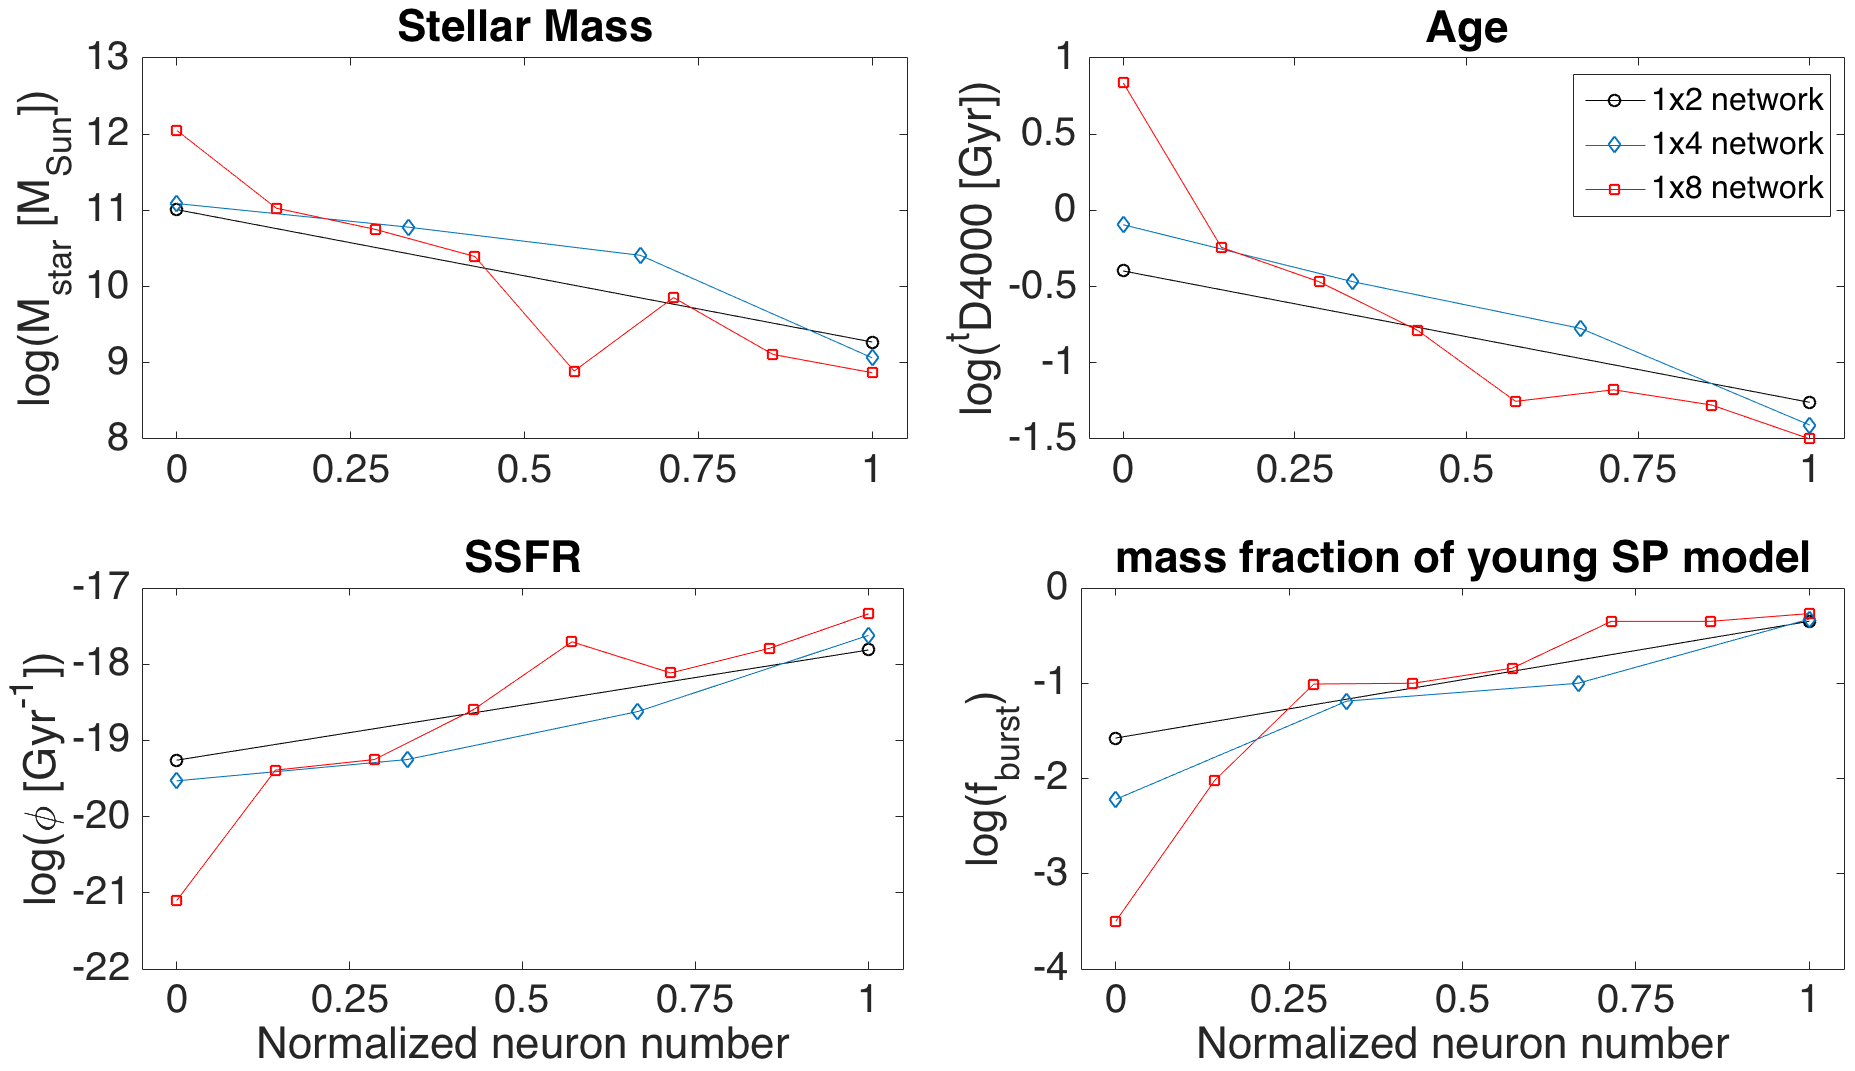
\includegraphics[width=0.5\textwidth]{images0.01/1d/props5.png}
            \caption{Median values of four properties of galaxies in each node in $1\times2$ (black circles), $1\times4$ (blue diamonds), and $1\times8$ (red triangles) networks.}
            \label{fig: props}
        \end{figure}
       
        Fig.~\ref{fig: props} shows the median values of stellar mass, age, specific star formation rate (sSFR; star formation rate per stellar mass), and $f_\mathrm{burst}$ of the galaxies in each neuron in the $1\times2$, $1\times4$, and $1\times8$ networks.
        In all plots, the horizontal axis is the number of the neurons divided by the size of the network.
        As shown in Fig.~\ref{fig: props}, in all three networks, stellar mass and age decrease while sSFR and $f_\mathrm{burst}$ increase as the type changes from early type galaxies to starburst. 
        Separating galaxies based on SED types also leads to a separation in properties that derived (via {\sc CIGALE}) from the SEDs, as expected since the SED types are also based on {\sc CIGALE} fitting. 
    
        {\sc CIGALE} has various models to derive the properties of galaxies.
        Through these models, some of the properties are already known to be correlated with each other, e.g., stellar mass and star formation rate.
        \citetalias{Noll09} studied other relations between properties with no direct correlation in the models in a sample of SINGS galaxies.
        They found a tight correlation between sSFR and t$_{\rm {D4000}}$, which suggests that younger stellar population correlates with higher SFR.
        They also found correlations between stellar mass and SFR, and stellar mass and t$_{\rm {D4000}}$.
        Since in the {\sc CIGALE} code, stellar mass is a free parameter, \citetalias{Noll09} argued that any stellar-mass-related correlation must be astrophysically meaningful. 
        They also studied relations between the attenuation at 1500 \AA~(A$_{\rm {FUV}}$) and sSFR, age, and stellar mass and did not find any correlation.
        \citetalias{Hossein12} replicated the upper plots in Fig.~\ref{fig: props_vs_props}, and found a tighter correlation than \citetalias{Noll09} results. 
        
               \begin{figure*}
        \begin{subfigure}[b]{0.3\textwidth}
            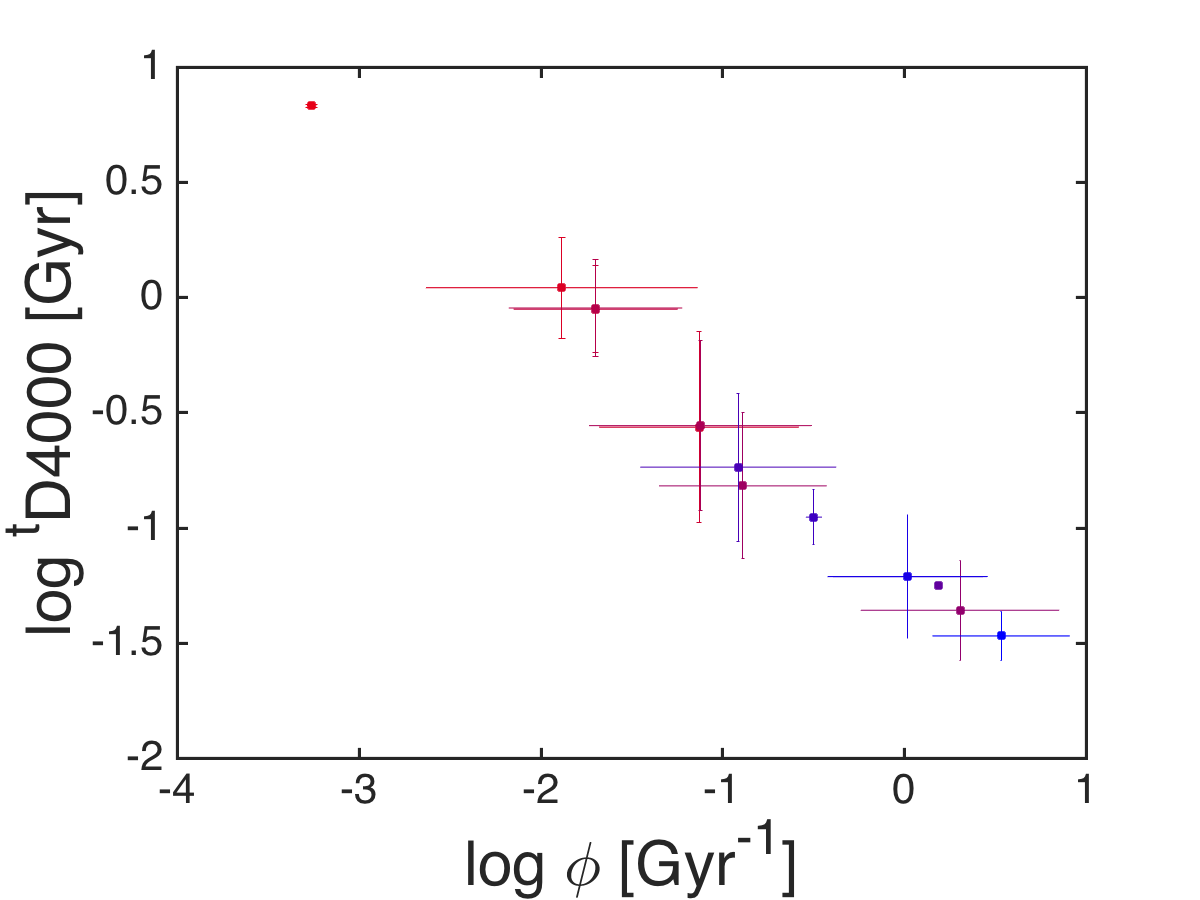
\includegraphics[width=\textwidth]{images0.01/1d/f1.png}
        \end{subfigure}
        \hfill
        \begin{subfigure}[b]{0.3\textwidth}
            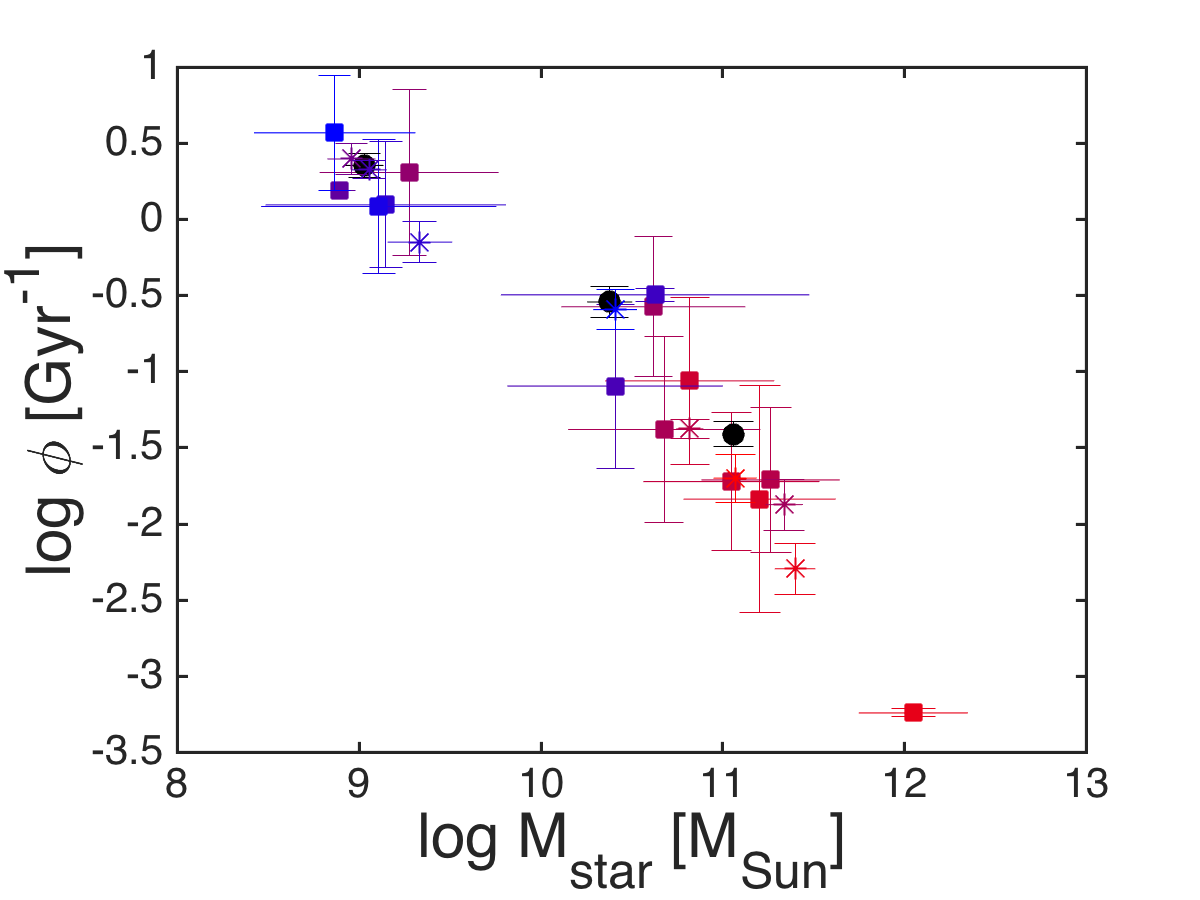
\includegraphics[width=\textwidth]{images0.01/1d/f2.png}
        \end{subfigure}
        \hfill
        \begin{subfigure}[b]{0.3\textwidth}
            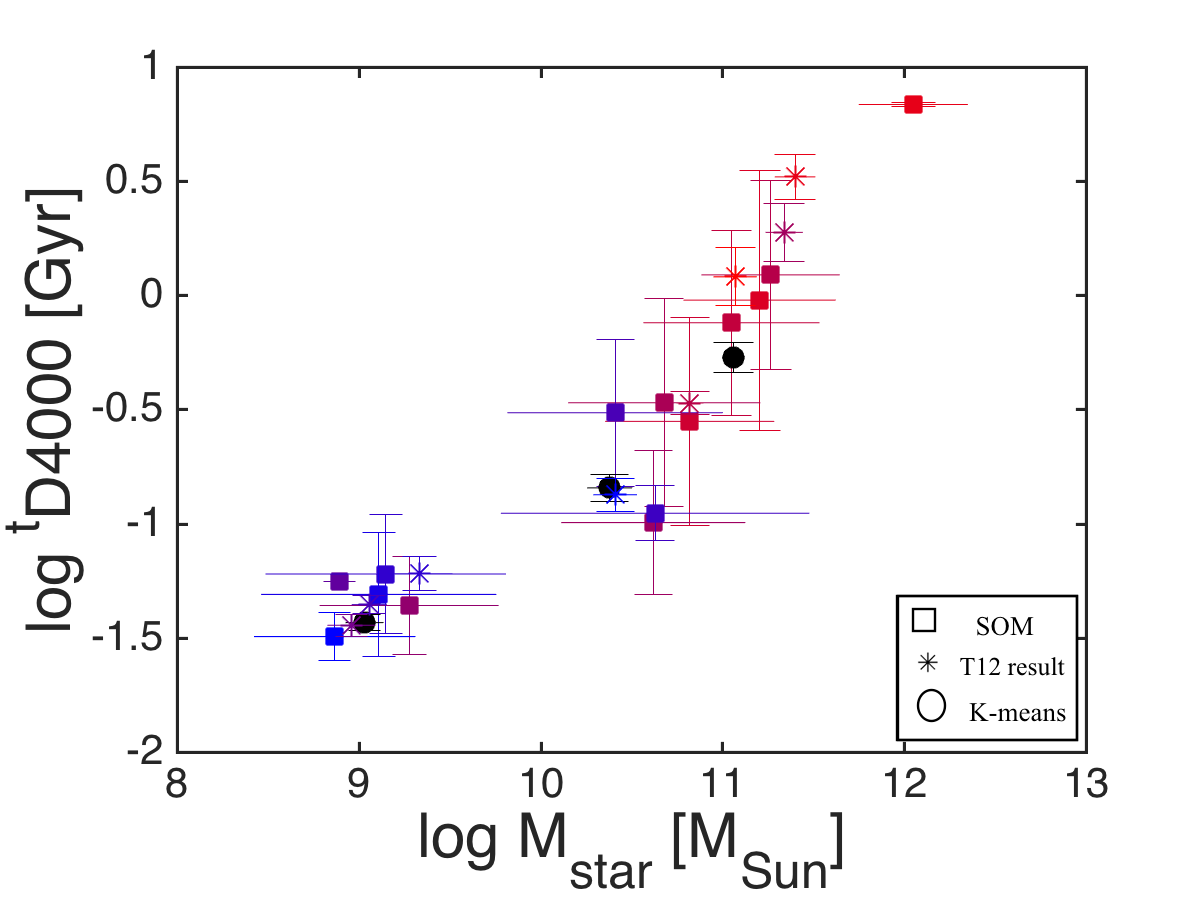
\includegraphics[width=\textwidth]{images0.01/1d/f3.png}
        \end{subfigure}
        \hfill
        \begin{subfigure}[b]{0.3\textwidth}
            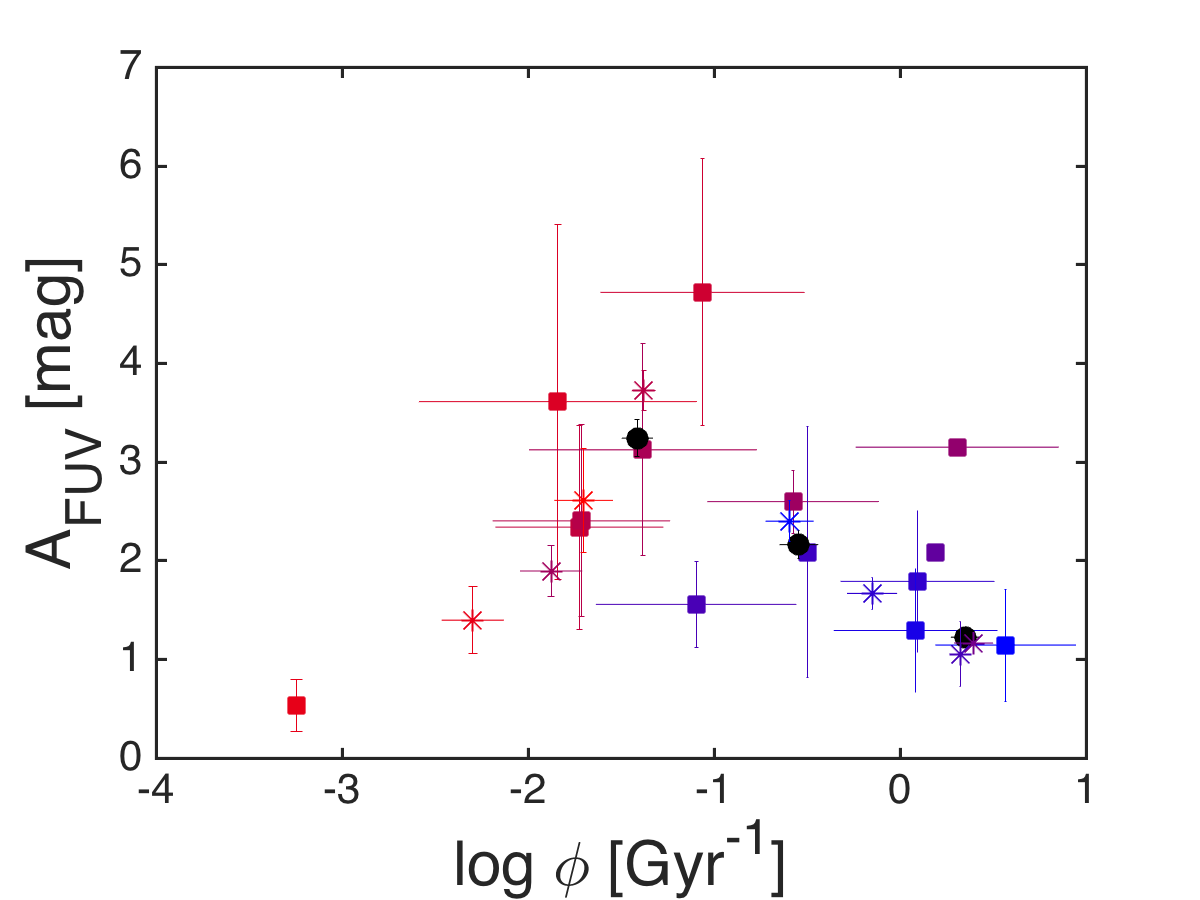
\includegraphics[width=\textwidth]{images0.01/1d/f4.png}
        \end{subfigure}
        \hfill
        \begin{subfigure}[b]{0.3\textwidth}
            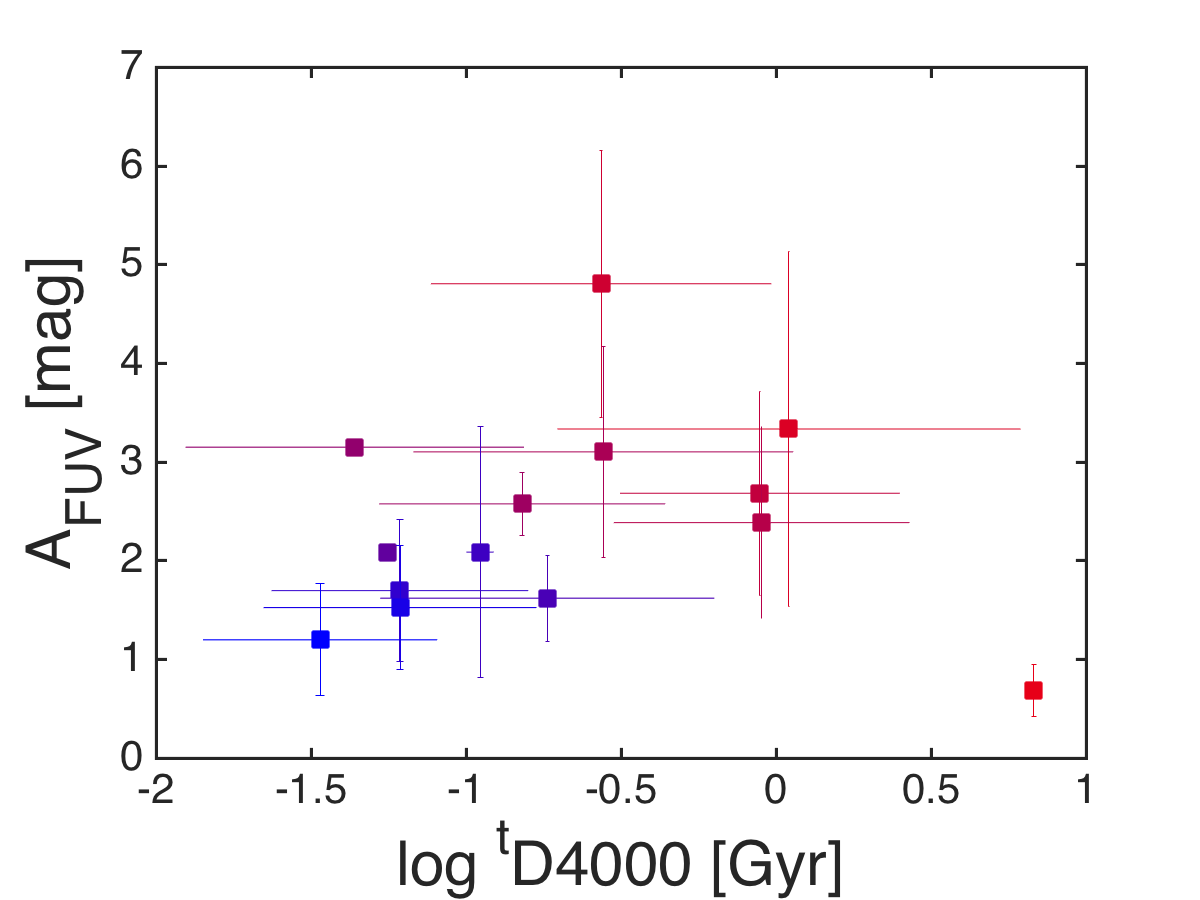
\includegraphics[width=\textwidth]{images0.01/1d/f5.png}
        \end{subfigure}
       \hfill
        \begin{subfigure}[b]{0.3\textwidth}
            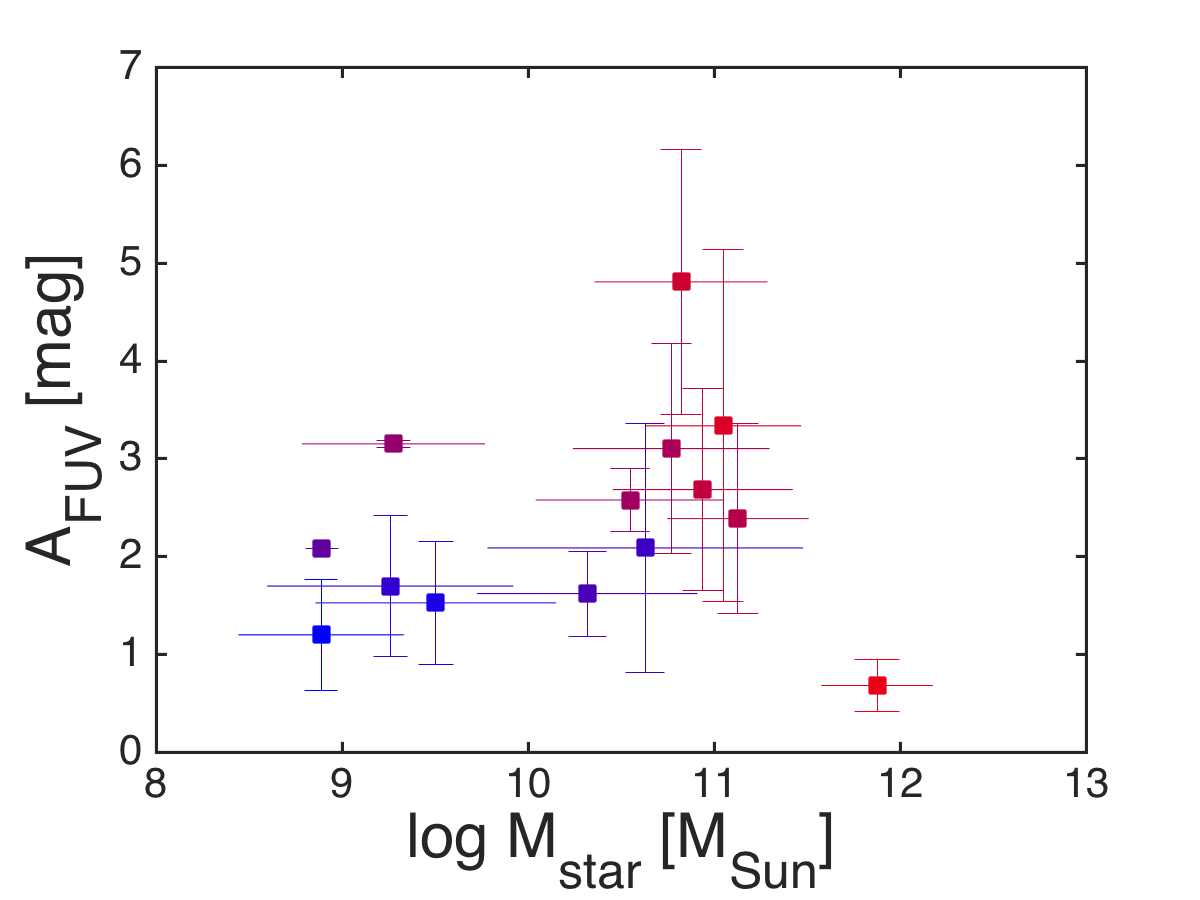
\includegraphics[width=\textwidth]{images0.01/1d/f6.png}
        \end{subfigure}
        \caption{From top to bottom: Correlation between age (t$_{\rm {D4000}}$) and sSFR ($\phi$), sSFR and stellar mass, age (t$_{\rm {D4000}}$) and stellar mass, and A$_{\rm {FUV}}$ with sSFR, age (t$_{\rm {D4000}}$) and stellar mass. Points show the median values of these properties of galaxies in the $1\times22$ network and error bars are the standard deviation of the median values. Colours show the type of galaxies in the new classification. The purest red colour shows E type galaxies and the bluest one indicates the SB1 galaxies. The other colours are determined by the galaxy group's relative distance to these two endpoints.}
        \label{fig: props_vs_props}
    \end{figure*}
        
        In order to compare our classifications with previous works, we produced similar plots to the ones in both \citetalias{Noll09} and \citetalias{Hossein12} (Fig.~\ref{fig: props_vs_props}).
        In Fig.~\ref{fig: props_vs_props}, the data points are median values of the properties of the galaxies in each neuron in Fig.~\ref{fig: 1by22V}, and error bars show the standard deviation of those properties.
        The colours show the galaxy types, where B type galaxies are shown with red and SB1 types are shown with blue.
        The redder the colour, the more similarity with  quiescent galaxies, while the purple to blue colours show more similarity to starburst galaxies.
        Since in this method we allow galaxies to occupy classes in between the original \citetalias{Kinney96} templates, we have more than 12 colours in Fig.~\ref{fig: props_vs_props}.
        The purple point in the middle of the blue points in  Fig.~\ref{fig: props_vs_props} corresponds to galaxies with SEDs similar to type Sc: the shape of their SED indicates that they are old galaxies with high sSFR.
        
        The upper panels in Fig.~\ref{fig: props_vs_props} show the same relations as \citetalias{Noll09} and \citetalias{Hossein12}, but with tighter correlation than those two, in all three plots.
        As mentioned in both \citetalias{Noll09} and \citetalias{Hossein12}, galaxies with smaller mass tend to be younger and more active.
        Fig.~\ref{fig: props} shows similar results: younger and more active galaxies have less stellar mass and more f$_{\rm {burst}}$.
        From older to younger galaxies, the colour of the points changes from red to blue, which shows a good correlation with their SED type.
       
        \citetalias{Noll09} studied a correlation between A$_{\rm {FUV}}$ and other properties of galaxies and showed that the attenuation has no dependence on the specific star formation or age.
        In contrast to \citetalias{Noll09}, we find a correlation between A$_{\rm {FUV}}$ and these two parameters, shown in the lower panels of Fig.~\ref{fig: props_vs_props}.
        The general trend of the correlation between A$_{\rm {FUV}}$ and sSFR in Fig.~\ref{fig: props_vs_props} is similar to the trend found by \cite{Dale07}.
        They used IR luminosity to UV luminosity ratio (L$_{IR}$/L$_{FUV}$) as a measure of A$_{\rm {FUV}}$ and compared it with sSFR for all 75 galaxies in the SINGS survey.
        They found that for early type galaxies (E, S0 and S0/a ), L$_{IR}$/L$_{FUV}$ (or A$_{\rm {FUV}}$ ) correlates with sSFR, and for spiral galaxies, there is an anticorrelation between L$_{IR}$/L$_{FUV}$ and sSFR.
       Since our sample has no E-type galaxies, we cannot confidently show the same correlation between A$_{\rm {FUV}}$ and sSFR. 
        However, it is clear in Fig.~\ref{fig: props_vs_props} that A$_{\rm {FUV}}$ increases with increasing sSFR in the S0 and Sa types.
        The correlation in the other types of galaxies is very similar to the one shown by \cite{Dale07}.
        Both \cite{Dale07} and \citetalias{Noll09} argued that these apparent trends can be a result of the dependence of star formation history on L$_{IR}$/L$_{FUV}$.
        Whether this dependence is real or not, our results here show that using self-organizing maps can separate SEDs of galaxies in such a way that the characteristics of each of these groups are in agreement with the general picture of the galaxy evolution.
        
        
    \subsection{Two-dimensional self-organizing maps}
    \label{sec: 2D}
    One-dimensional networks are great tools to categorize the SEDs and monitor the changes of properties of galaxies with category.
    However, each neuron in these networks is limited to be connected to one other neuron in each direction.
    In a 2D network, each neuron can have more than two immediate neighbours, providing a more complete pictures of relations between SED types.
    As described in Sec.~\ref{sec: method}, one of the main advantages of the SOM is that when the weight of one neuron is adjusted after finding the best matching unit, the weight of the whole map will be changed.
    This quality of the SOMs provides a unique opportunity to analyse 2D networks in two approaches. 
    At first, as in the 1D SOMs, we assumed that all the galaxies must have SEDs similar to any of the 12 templates in Fig.~\ref{fig: k96}.
    In this case, we can categorize SEDs of other galaxies based on those 12 types.
   In the second approach, we trained networks with the assumption that there might be completely different types of galaxies not encountered before.
    This approach can be used to trace and recognize the outliers.
    To execute the second approach, we used the {\sc selforgmap} library in {\sc matlab}.
    Using the {\sc selforgmap} code, based on the size of a map and the ordering step neighbourhood distance, we can arrange that the data spread all over the SOM or sit close together, allowing room for outliers.

    To get the best result from both methods, we should have SOMs with ``enough"  neurons to give any new types of galaxies a chance to find their places in the map.
    ``Enough  neurons" is a vague statement, but as mentioned in Sec.~\ref{sec: method} the size of SOMs is arbitrary and depends on the size of the input data and the kind of information needed from the SOMs.
    Since the training dataset (the \citetalias{Kinney96} templates) has 12 members, we assumed a SOM with size of $8\times8$~would be a good start.
    We then increased the size of the SOM to find the highest size suitable for the training sample.
    We noticed that very few changes occurred after the SOMs were grown to a size greater than $12\times12$, so we used this as the maximum size.
    
    \begin{figure*}
        \begin{subfigure}[b]{0.45\textwidth}
            \centering
            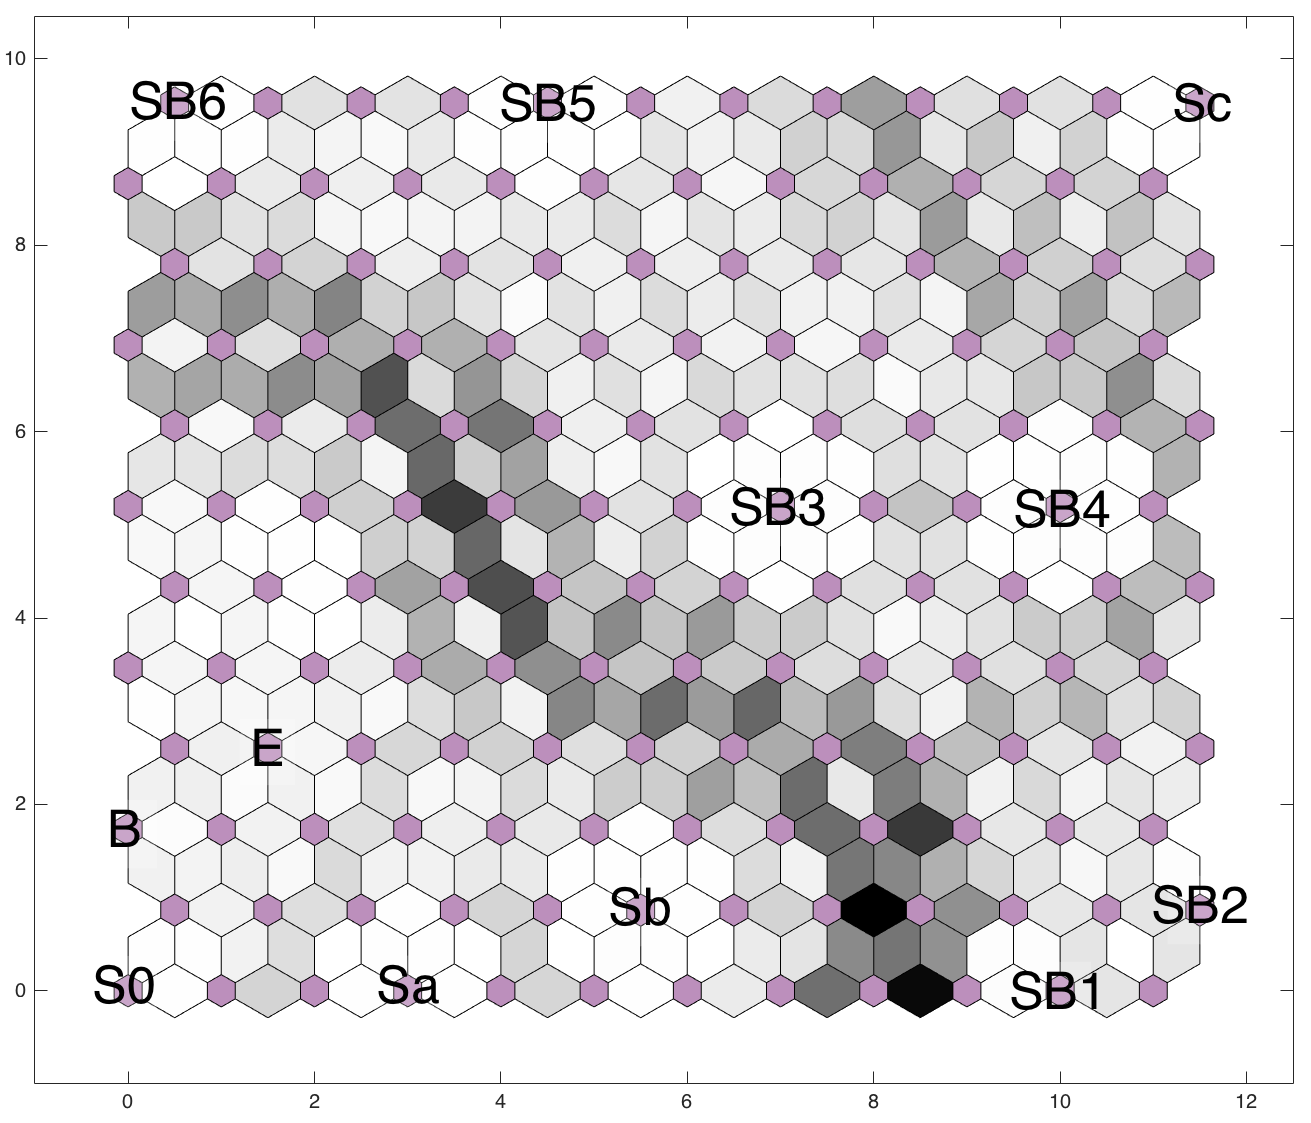
\includegraphics[width=\textwidth]{images0.01/2d/dist_12_by_12.png}
        \end{subfigure}
        \hfill
        \begin{subfigure}[b]{0.45\textwidth}
            \centering
            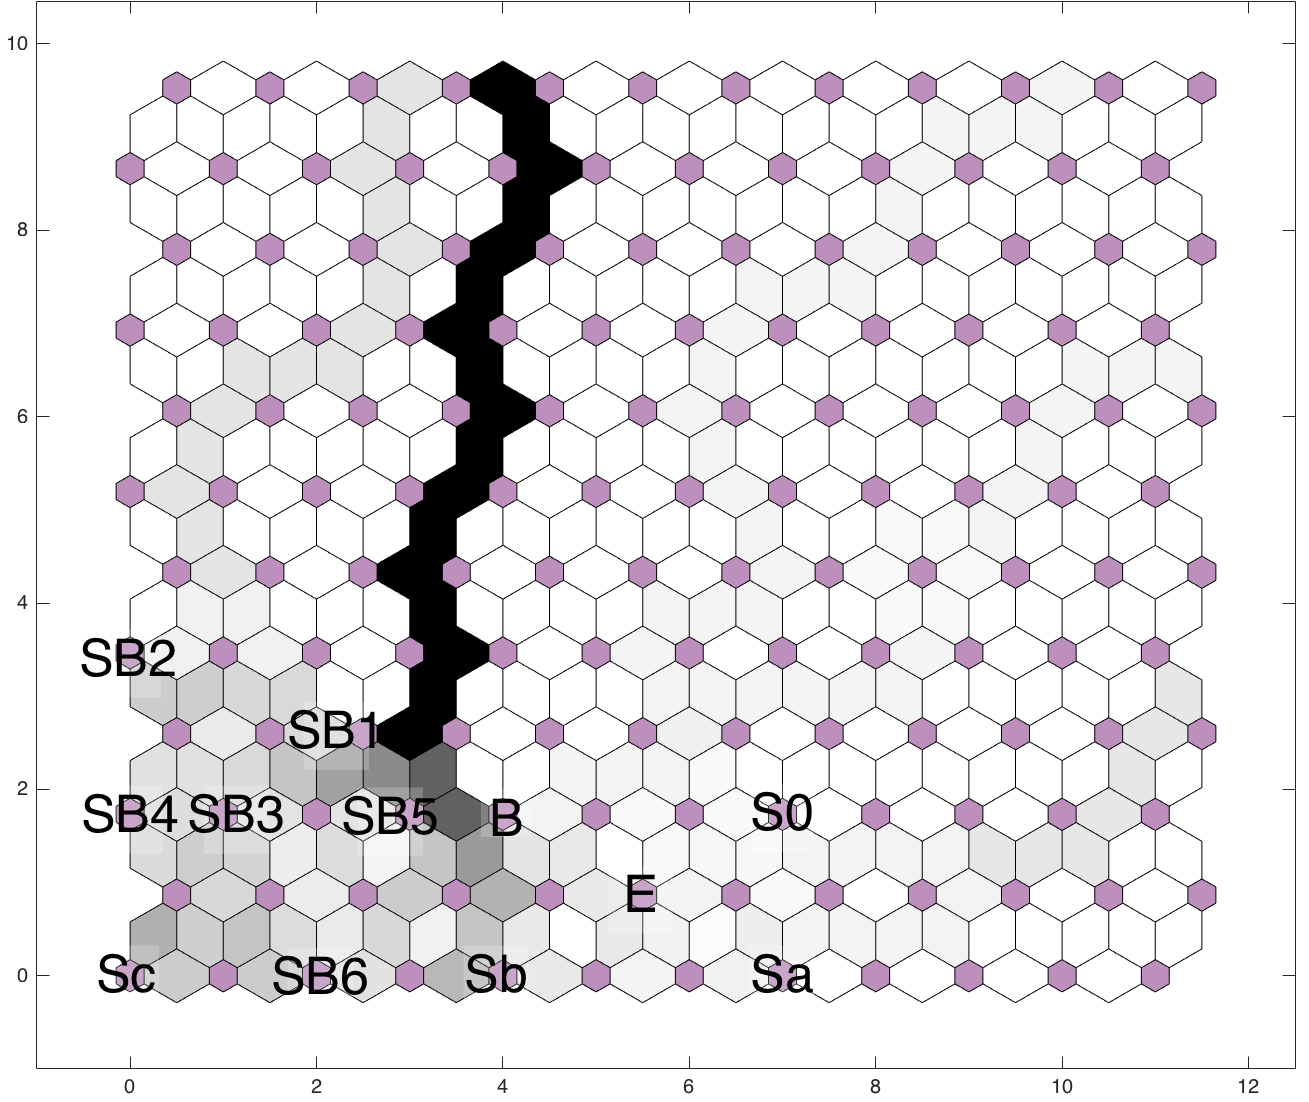
\includegraphics[width=\textwidth]{images0.01/2d/dist_12_by_self_org_res12.png}
        \end{subfigure}
        \hfill
        \begin{subfigure}[b]{0.45\textwidth}
            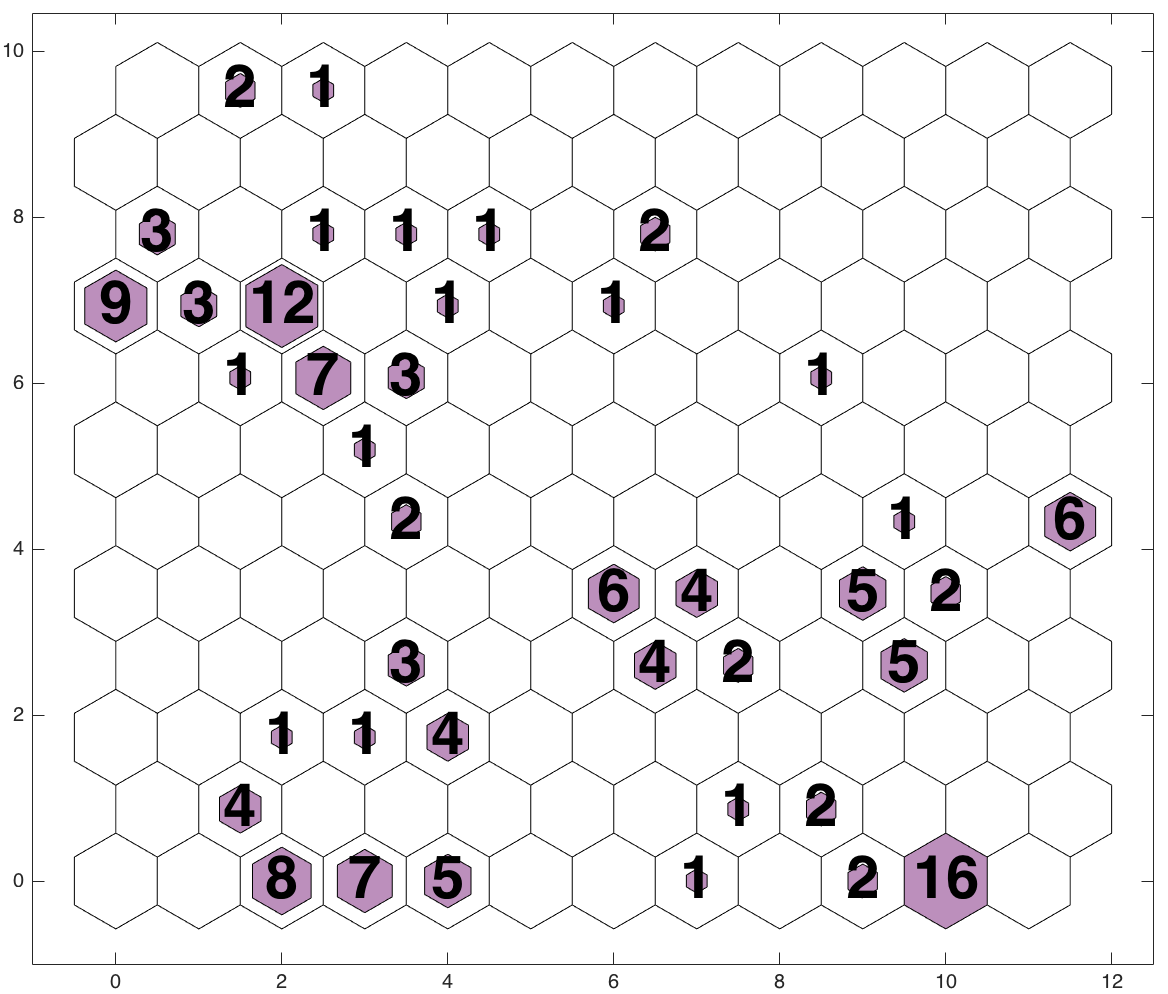
\includegraphics[width=\textwidth]{images0.01/2d/hit_v_12_by_12.png}
        \end{subfigure}
        \hfill
        \begin{subfigure}[b]{0.45\textwidth}
            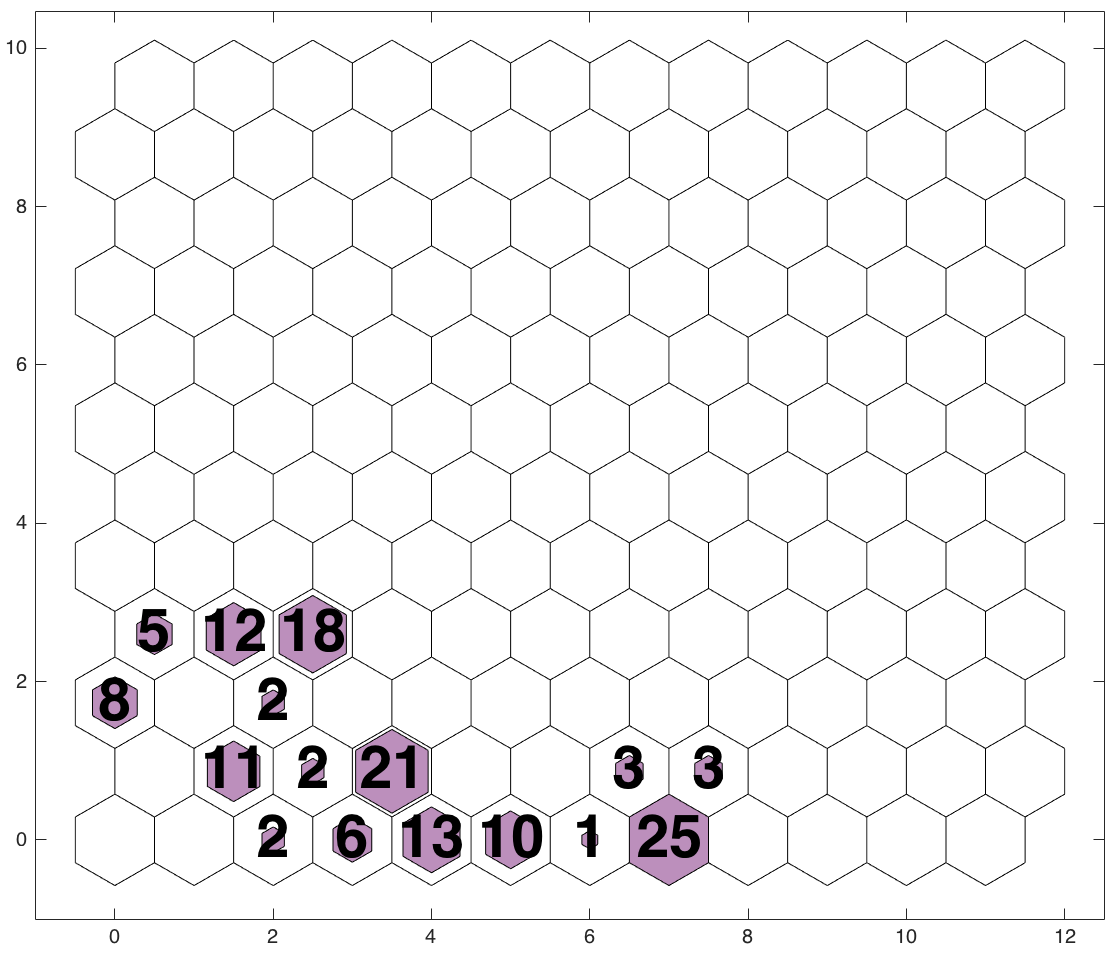
\includegraphics[width=\textwidth]{images0.01/2d/hit_v_12_by_self_org_res12.png}
        \end{subfigure}
        \caption{$12\times12$~2D SOM results. Upper panel: SOMs trained using the \citetalias{Kinney96} templates. For training 2D SOMs two different approaches were considered: either only 12 types of galaxies exist (left) or not (right). Lower panel: classifying the galaxies from \citetalias{Hossein12}, using the trained networks shown in the upper panels. From the lower right panel, we can see that there are no outliers in the galaxies from \citetalias{Hossein12}, and we can use the map in the lower left panel as a final clustering result for the \citetalias{Hossein12} galaxies.}
        \label{fig: 12by12}
    \end{figure*}
    
    The upper left panel in Fig.~\ref{fig: 12by12} shows the SOM results from the first approach. 
    Since we considered that SEDs of all galaxies can be categorized using the \citetalias{Kinney96} templates, the galaxies were placed all over the map.
    Using this network to categorize any set of SEDs forced the SEDs to be either in the same neurons as the \citetalias{Kinney96} templates or in the neurons between them.
    In the map shown in the upper right panel in Fig.~\ref{fig: 12by12}, the \citetalias{Kinney96} templates are in a small region. This provides enough freedom for the SEDs of galaxies to be placed everywhere in the map, even far away from the templates.
    
    
    In the upper left part of the map in Fig.~\ref{fig: 12by12}, although galaxies have more ways to be separated, they were separated in two main groups.
    There is a distinguishable strip of grey, dark grey and in some cases black colour in the map:
    this strip separates quiescent galaxies from starburst ones.
    The lower map shows that 5 of the neurons on the left side of the strip are full. 
    These five neurons are the same as the ones on the left hand side of Fig.~\ref{fig: 1by2T},
    the only difference being that in this map they have more space to be separated from each other.
    When we use this network to categorize the SED of galaxies, any galaxy placed on the left hand side of the strip is a quiescent galaxy and any one placed on the right side of the strip is a starburst one.
    The decision about what sub-type of early type or starburst galaxy is based upon its relative position to each type in the SOM.
    
    As in the other map, in the upper right panel of Fig.~\ref{fig: 12by12}, galaxies are generally divided into two main groups.
    The border between the early type galaxies and the starburst ones is the black strips in the middle of the map,  ending with the bright grey colour at the bottom of the map in the fifth neuron.
    In this network, neurons in the right side of the strip represent the quiescent galaxies and the neurons in the left side represent the starburst ones. 
    When categorizing a new set of SEDs, if the new SEDs are similar to the \citetalias{Kinney96} template all of them will be placed in the bottom of the map, but if there are different type of galaxies, they would sit in any other neurons in the map.
    In large datasets, one can easily use this network to determine whether there is any new type of SEDs (or any outliers) in the datasets. 
    Since the networks are already available, this procedure should be quick and easy for large datasets.
    
    We used both 2D networks to categorize the \citetalias{Hossein12} galaxies and the results are shown in the lower panels of Fig.~\ref{fig: 12by12}.
    In the lower right map in Fig.~\ref{fig: 12by12}, all galaxies are placed in the bottom part of the map and we can conclude that in the \citetalias{Hossein12} sample there are no outliers or SEDs very different from  the \citetalias{Kinney96} templates.
    The lower left map of Fig.~\ref{fig: 12by12} shows the \citetalias{Hossein12} galaxies categorized based on the network in the upper left of Fig.~\ref{fig: 12by12}. 
    Comparing this categorization with the 1D one from Fig.~\ref{fig: 1by22V}, we can see that only 23 galaxies correspond exactly to \citetalias{Kinney96} types.
    Using 2D maps results in categorizing galaxies into more intermediate type than in 1D maps.
    In both lower maps in Fig.~\ref{fig: 12by12}, most galaxies are in the quiescent side of the SOM, which was predictable from the results in Sec.\ref{sec: 1Dv}. This does not imply that in general there are more quiescent galaxies at higher red-shifts but rather is a selection effect from the fact that those galaxies had more reliable redshift estimates.
    
    Although for ease of presentation this paper first discusses 1D networks and continues to 2D networks, we suggest that users of SOMs for galaxy SED classification should use 2D networks first. These can be used as a first step with networks similar to the upper left map in Fig.~\ref{fig: 12by12} to identify outliers in the sample.